\documentclass[a4paper]{book}
\usepackage{a4wide}
\usepackage{makeidx}
\usepackage{graphicx}
\usepackage{multicol}
\usepackage{float}
\usepackage{listings}
\usepackage{color}
\usepackage{textcomp}
\usepackage{alltt}
\usepackage{times}
\usepackage{ifpdf}
\ifpdf
\usepackage[pdftex,
            pagebackref=true,
            colorlinks=true,
            linkcolor=blue,
            unicode
           ]{hyperref}
\else
\usepackage[ps2pdf,
            pagebackref=true,
            colorlinks=true,
            linkcolor=blue,
            unicode
           ]{hyperref}
\usepackage{pspicture}
\fi
\usepackage[utf8]{inputenc}
\usepackage{doxygen}
\lstset{language=C++,inputencoding=utf8,basicstyle=\footnotesize,breaklines=true,breakatwhitespace=true,tabsize=8,numbers=left }
\makeindex
\setcounter{tocdepth}{3}
\renewcommand{\footrulewidth}{0.4pt}
\begin{document}
\hypersetup{pageanchor=false}
\begin{titlepage}
\vspace*{7cm}
\begin{center}
{\Large Reference Manual}\\
\vspace*{1cm}
{\large Generated by Doxygen 1.6.1}\\
\vspace*{0.5cm}
{\small Tue May 17 20:09:09 2011}\\
\end{center}
\end{titlepage}
\clearemptydoublepage
\pagenumbering{roman}
\tableofcontents
\clearemptydoublepage
\pagenumbering{arabic}
\hypersetup{pageanchor=true}
\chapter{Class Index}
\section{Class Hierarchy}
This inheritance list is sorted roughly, but not completely, alphabetically:\begin{DoxyCompactList}
\item \contentsline{section}{asfig}{\pageref{structasfig}}{}
\item \contentsline{section}{asisc}{\pageref{structasisc}}{}
\item \contentsline{section}{asiss}{\pageref{structasiss}}{}
\item \contentsline{section}{asobj}{\pageref{structasobj}}{}
\item \contentsline{section}{asosc}{\pageref{structasosc}}{}
\item \contentsline{section}{Basic\_\-block}{\pageref{classBasic__block}}{}
\item \contentsline{section}{Function}{\pageref{classFunction}}{}
\item \contentsline{section}{Line}{\pageref{classLine}}{}
\begin{DoxyCompactList}
\item \contentsline{section}{Directive}{\pageref{classDirective}}{}
\item \contentsline{section}{Instruction}{\pageref{classInstruction}}{}
\item \contentsline{section}{Label}{\pageref{classLabel}}{}
\end{DoxyCompactList}
\item \contentsline{section}{Node}{\pageref{classNode}}{}
\item \contentsline{section}{Operand}{\pageref{classOperand}}{}
\begin{DoxyCompactList}
\item \contentsline{section}{OPExpression}{\pageref{classOPExpression}}{}
\item \contentsline{section}{OPImmediate}{\pageref{classOPImmediate}}{}
\item \contentsline{section}{OPLabel}{\pageref{classOPLabel}}{}
\item \contentsline{section}{OPRegister}{\pageref{classOPRegister}}{}
\end{DoxyCompactList}
\item \contentsline{section}{Program}{\pageref{classProgram}}{}
\item \contentsline{section}{s\_\-Profile}{\pageref{structs__Profile}}{}
\item \contentsline{section}{TestOPLabel}{\pageref{classTestOPLabel}}{}
\item \contentsline{section}{utchn}{\pageref{structutchn}}{}
\item \contentsline{section}{utdat}{\pageref{unionutdat}}{}
\item \contentsline{section}{utdic}{\pageref{structutdic}}{}
\item \contentsline{section}{utdit}{\pageref{structutdit}}{}
\item \contentsline{section}{uttdc}{\pageref{structuttdc}}{}
\item \contentsline{section}{uttpd}{\pageref{structuttpd}}{}
\item \contentsline{section}{uttyp}{\pageref{structuttyp}}{}
\item \contentsline{section}{YYSTYPE}{\pageref{unionYYSTYPE}}{}
\end{DoxyCompactList}

\chapter{Class Index}
\section{Class List}
Here are the classes, structs, unions and interfaces with brief descriptions:\begin{DoxyCompactList}
\item\contentsline{section}{\hyperlink{structasfig}{asfig} }{\pageref{structasfig}}{}
\item\contentsline{section}{\hyperlink{structasisc}{asisc} }{\pageref{structasisc}}{}
\item\contentsline{section}{\hyperlink{structasiss}{asiss} }{\pageref{structasiss}}{}
\item\contentsline{section}{\hyperlink{structasobj}{asobj} }{\pageref{structasobj}}{}
\item\contentsline{section}{\hyperlink{structasosc}{asosc} }{\pageref{structasosc}}{}
\item\contentsline{section}{\hyperlink{classBasic__block}{Basic\_\-block} (Class representing a \hyperlink{classBasic__block}{Basic\_\-block} of a fonction )}{\pageref{classBasic__block}}{}
\item\contentsline{section}{\hyperlink{classDirective}{Directive} (Class representing an \hyperlink{classDirective}{Directive} herited by \hyperlink{classLine}{Line} )}{\pageref{classDirective}}{}
\item\contentsline{section}{\hyperlink{classFunction}{Function} (Class representing a \hyperlink{classFunction}{Function} on a program )}{\pageref{classFunction}}{}
\item\contentsline{section}{\hyperlink{classInstruction}{Instruction} (Class representing an instruction which herited by \hyperlink{classLine}{Line} )}{\pageref{classInstruction}}{}
\item\contentsline{section}{\hyperlink{classLabel}{Label} (Class representing an \hyperlink{classLabel}{Label} herited by \hyperlink{classLine}{Line} )}{\pageref{classLabel}}{}
\item\contentsline{section}{\hyperlink{classLine}{Line} (Abstract class representing an \hyperlink{classLine}{Line} )}{\pageref{classLine}}{}
\item\contentsline{section}{\hyperlink{classNode}{Node} (Class representing a \hyperlink{classNode}{Node} in list )}{\pageref{classNode}}{}
\item\contentsline{section}{\hyperlink{classOperand}{Operand} (Abstract class representing an operand )}{\pageref{classOperand}}{}
\item\contentsline{section}{\hyperlink{classOPExpression}{OPExpression} (Class representing an expression herited by \hyperlink{classOperand}{Operand} )}{\pageref{classOPExpression}}{}
\item\contentsline{section}{\hyperlink{classOPImmediate}{OPImmediate} (Class representing an Immediate herited by \hyperlink{classOperand}{Operand} )}{\pageref{classOPImmediate}}{}
\item\contentsline{section}{\hyperlink{classOPLabel}{OPLabel} (Class representing a \hyperlink{classLabel}{Label} herited by \hyperlink{classOperand}{Operand} )}{\pageref{classOPLabel}}{}
\item\contentsline{section}{\hyperlink{classOPRegister}{OPRegister} (Class representing a Register herited by \hyperlink{classOperand}{Operand} )}{\pageref{classOPRegister}}{}
\item\contentsline{section}{\hyperlink{classProgram}{Program} (Class representing a program as list )}{\pageref{classProgram}}{}
\item\contentsline{section}{\hyperlink{structs__Profile}{s\_\-Profile} (Structure allowing to add caracteristics to an operator )}{\pageref{structs__Profile}}{}
\item\contentsline{section}{\hyperlink{classTestOPLabel}{TestOPLabel} }{\pageref{classTestOPLabel}}{}
\item\contentsline{section}{\hyperlink{structutchn}{utchn} }{\pageref{structutchn}}{}
\item\contentsline{section}{\hyperlink{unionutdat}{utdat} }{\pageref{unionutdat}}{}
\item\contentsline{section}{\hyperlink{structutdic}{utdic} }{\pageref{structutdic}}{}
\item\contentsline{section}{\hyperlink{structutdit}{utdit} }{\pageref{structutdit}}{}
\item\contentsline{section}{\hyperlink{structuttdc}{uttdc} }{\pageref{structuttdc}}{}
\item\contentsline{section}{\hyperlink{structuttpd}{uttpd} }{\pageref{structuttpd}}{}
\item\contentsline{section}{\hyperlink{structuttyp}{uttyp} }{\pageref{structuttyp}}{}
\item\contentsline{section}{\hyperlink{unionYYSTYPE}{YYSTYPE} }{\pageref{unionYYSTYPE}}{}
\end{DoxyCompactList}

\chapter{File Index}
\section{File List}
Here is a list of all documented files with brief descriptions:\begin{DoxyCompactList}
\item\contentsline{section}{{\bfseries asm200.h} }{\pageref{asm200_8h}}{}
\item\contentsline{section}{{\bfseries asm\_\-mipsyac.h} }{\pageref{asm__mipsyac_8h}}{}
\item\contentsline{section}{\hyperlink{Basic__block_8h}{Basic\_\-block.h} (\hyperlink{classBasic__block}{Basic\_\-block} class )}{\pageref{Basic__block_8h}}{}
\item\contentsline{section}{\hyperlink{Directive_8h}{Directive.h} (\hyperlink{classDirective}{Directive} class )}{\pageref{Directive_8h}}{}
\item\contentsline{section}{{\bfseries Enum\_\-type.h} }{\pageref{Enum__type_8h}}{}
\item\contentsline{section}{\hyperlink{Function_8h}{Function.h} (\hyperlink{classFunction}{Function} class )}{\pageref{Function_8h}}{}
\item\contentsline{section}{\hyperlink{Instruction_8h}{Instruction.h} (\hyperlink{classInstruction}{Instruction} class )}{\pageref{Instruction_8h}}{}
\item\contentsline{section}{\hyperlink{Label_8h}{Label.h} (\hyperlink{classLabel}{Label} class )}{\pageref{Label_8h}}{}
\item\contentsline{section}{\hyperlink{Line_8h}{Line.h} (\hyperlink{classLine}{Line} class )}{\pageref{Line_8h}}{}
\item\contentsline{section}{\hyperlink{Node_8h}{Node.h} (\hyperlink{classNode}{Node} class )}{\pageref{Node_8h}}{}
\item\contentsline{section}{\hyperlink{Operand_8h}{Operand.h} (\hyperlink{classOperand}{Operand} class )}{\pageref{Operand_8h}}{}
\item\contentsline{section}{\hyperlink{OPExpression_8h}{OPExpression.h} (\hyperlink{classOPExpression}{OPExpression} class )}{\pageref{OPExpression_8h}}{}
\item\contentsline{section}{\hyperlink{OPImmediate_8h}{OPImmediate.h} (\hyperlink{classOPImmediate}{OPImmediate} class )}{\pageref{OPImmediate_8h}}{}
\item\contentsline{section}{\hyperlink{OPLabel_8h}{OPLabel.h} (\hyperlink{classOPLabel}{OPLabel} class )}{\pageref{OPLabel_8h}}{}
\item\contentsline{section}{\hyperlink{OPRegister_8h}{OPRegister.h} (\hyperlink{classOPRegister}{OPRegister} class )}{\pageref{OPRegister_8h}}{}
\item\contentsline{section}{\hyperlink{Program_8h}{Program.h} (\hyperlink{classProgram}{Program} class )}{\pageref{Program_8h}}{}
\item\contentsline{section}{{\bfseries TestOPLabel.h} }{\pageref{TestOPLabel_8h}}{}
\item\contentsline{section}{{\bfseries utl200.h} }{\pageref{utl200_8h}}{}
\end{DoxyCompactList}

\chapter{Class Documentation}
\hypertarget{structasfig}{
\section{asfig Struct Reference}
\label{structasfig}\index{asfig@{asfig}}
}
\subsection*{Public Attributes}
\begin{DoxyCompactItemize}
\item 
\hypertarget{structasfig_acb2f83dbe7a1e3cc29529820c2d84f08}{
struct \hyperlink{structutdic}{utdic} $\ast$ {\bfseries GLB\_\-DIC}}
\label{structasfig_acb2f83dbe7a1e3cc29529820c2d84f08}

\item 
\hypertarget{structasfig_a0d08a06c7ef0d7d128b068e63ec65a08}{
struct \hyperlink{structuttyp}{uttyp} $\ast$ {\bfseries GLB\_\-SYM}}
\label{structasfig_a0d08a06c7ef0d7d128b068e63ec65a08}

\item 
\hypertarget{structasfig_ae87202e68aa58ff7cf9d39b476d81d13}{
struct \hyperlink{structuttyp}{uttyp} $\ast$ {\bfseries MEM\_\-TAB}}
\label{structasfig_ae87202e68aa58ff7cf9d39b476d81d13}

\item 
\hypertarget{structasfig_a29babddc26cd0b8fec9c3c139dd78206}{
struct \hyperlink{structasosc}{asosc} $\ast$ {\bfseries OUT\_\-SEC}}
\label{structasfig_a29babddc26cd0b8fec9c3c139dd78206}

\item 
\hypertarget{structasfig_acdd790bc6a90c1a53d9c96d651d515ae}{
struct \hyperlink{structasisc}{asisc} $\ast$ {\bfseries IN\_\-SEC}}
\label{structasfig_acdd790bc6a90c1a53d9c96d651d515ae}

\item 
\hypertarget{structasfig_a7811bcfbf0a2fd6c47b0f457875d1379}{
struct \hyperlink{structasobj}{asobj} $\ast$ {\bfseries OBJECTS}}
\label{structasfig_a7811bcfbf0a2fd6c47b0f457875d1379}

\item 
\hypertarget{structasfig_aef8acd1ebd4a06c7be326a16a3d587fc}{
unsigned int {\bfseries FLAG}}
\label{structasfig_aef8acd1ebd4a06c7be326a16a3d587fc}

\end{DoxyCompactItemize}


The documentation for this struct was generated from the following file:\begin{DoxyCompactItemize}
\item 
asm200.h\end{DoxyCompactItemize}

\hypertarget{structasisc}{
\section{asisc Struct Reference}
\label{structasisc}\index{asisc@{asisc}}
}
\subsection*{Public Attributes}
\begin{DoxyCompactItemize}
\item 
\hypertarget{structasisc_ad9e1171351b4def0dee34a931bef06c2}{
struct \hyperlink{structasisc}{asisc} $\ast$ {\bfseries NEXT}}
\label{structasisc_ad9e1171351b4def0dee34a931bef06c2}

\item 
\hypertarget{structasisc_a556fa34f54b5c9c75dd76650538afc1d}{
char $\ast$ {\bfseries IDENT}}
\label{structasisc_a556fa34f54b5c9c75dd76650538afc1d}

\item 
\hypertarget{structasisc_a719068c36a0e9705bf73ee2f073c423d}{
struct \hyperlink{structasosc}{asosc} $\ast$ {\bfseries OUT\_\-SEC}}
\label{structasisc_a719068c36a0e9705bf73ee2f073c423d}

\item 
\hypertarget{structasisc_a2d489dd1bf43e16f31806a7e22b4c944}{
unsigned int {\bfseries POSITION}}
\label{structasisc_a2d489dd1bf43e16f31806a7e22b4c944}

\item 
\hypertarget{structasisc_acbc421dc86cceaf4736c520ab2380d76}{
unsigned int {\bfseries FLAG}}
\label{structasisc_acbc421dc86cceaf4736c520ab2380d76}

\end{DoxyCompactItemize}


The documentation for this struct was generated from the following file:\begin{DoxyCompactItemize}
\item 
asm200.h\end{DoxyCompactItemize}

\hypertarget{structasiss}{
\section{asiss Struct Reference}
\label{structasiss}\index{asiss@{asiss}}
}
\subsection*{Public Attributes}
\begin{DoxyCompactItemize}
\item 
\hypertarget{structasiss_a68628730acb005ea7f11ea68de1d0548}{
struct \hyperlink{structasiss}{asiss} $\ast$ {\bfseries NEXT}}
\label{structasiss_a68628730acb005ea7f11ea68de1d0548}

\item 
\hypertarget{structasiss_a80a8a734b96c46174e20eafa5fd2858b}{
unsigned int {\bfseries ADDR}}
\label{structasiss_a80a8a734b96c46174e20eafa5fd2858b}

\item 
\hypertarget{structasiss_ae165bd0b21aa1165d33a69e641103589}{
unsigned int {\bfseries SIZE}}
\label{structasiss_ae165bd0b21aa1165d33a69e641103589}

\item 
\hypertarget{structasiss_a359354e07893109790b9d08a4abd01ad}{
unsigned int {\bfseries FLAG}}
\label{structasiss_a359354e07893109790b9d08a4abd01ad}

\end{DoxyCompactItemize}


The documentation for this struct was generated from the following file:\begin{DoxyCompactItemize}
\item 
asm200.h\end{DoxyCompactItemize}

\hypertarget{structasobj}{
\section{asobj Struct Reference}
\label{structasobj}\index{asobj@{asobj}}
}
\subsection*{Public Attributes}
\begin{DoxyCompactItemize}
\item 
\hypertarget{structasobj_a9640c87bee0faf9f3f4e27464446b7dd}{
struct \hyperlink{structasobj}{asobj} $\ast$ {\bfseries NEXT}}
\label{structasobj_a9640c87bee0faf9f3f4e27464446b7dd}

\item 
\hypertarget{structasobj_ac3a92c991065cf1151dbe25b5db8166c}{
char $\ast$ {\bfseries IDENT}}
\label{structasobj_ac3a92c991065cf1151dbe25b5db8166c}

\item 
\hypertarget{structasobj_ae2c40a301646b04f58c3176b2059aa3f}{
struct \hyperlink{structutdic}{utdic} $\ast$ {\bfseries SYM\_\-DIC}}
\label{structasobj_ae2c40a301646b04f58c3176b2059aa3f}

\item 
\hypertarget{structasobj_a0af182b30fad283aa3dbb32fa02f368b}{
struct \hyperlink{structuttyp}{uttyp} $\ast$ {\bfseries SEC\_\-SYM}}
\label{structasobj_a0af182b30fad283aa3dbb32fa02f368b}

\item 
\hypertarget{structasobj_aabba21bee06e84d00e257ac15339fcf3}{
unsigned int {\bfseries FLAG}}
\label{structasobj_aabba21bee06e84d00e257ac15339fcf3}

\end{DoxyCompactItemize}


The documentation for this struct was generated from the following file:\begin{DoxyCompactItemize}
\item 
asm200.h\end{DoxyCompactItemize}

\hypertarget{structasosc}{
\section{asosc Struct Reference}
\label{structasosc}\index{asosc@{asosc}}
}
\subsection*{Public Attributes}
\begin{DoxyCompactItemize}
\item 
\hypertarget{structasosc_a7ee21b53000a550b8aefb67b1c6e5f7f}{
struct \hyperlink{structasosc}{asosc} $\ast$ {\bfseries NEXT}}
\label{structasosc_a7ee21b53000a550b8aefb67b1c6e5f7f}

\item 
\hypertarget{structasosc_afc8abd23436b76f81cefb8aba492ead0}{
char $\ast$ {\bfseries IDENT}}
\label{structasosc_afc8abd23436b76f81cefb8aba492ead0}

\item 
\hypertarget{structasosc_a71acd15a4ac27fe271378a7ee411a703}{
unsigned int {\bfseries INS\_\-NBR}}
\label{structasosc_a71acd15a4ac27fe271378a7ee411a703}

\item 
\hypertarget{structasosc_a9839e2ff30cb42d4d0318b5ac52c1814}{
struct \hyperlink{structasiss}{asiss} $\ast$$\ast$ {\bfseries CUR\_\-ISS}}
\label{structasosc_a9839e2ff30cb42d4d0318b5ac52c1814}

\item 
\hypertarget{structasosc_abc1c84286924d8ea3a97a9374976d156}{
struct \hyperlink{structasiss}{asiss} $\ast$$\ast$ {\bfseries SUB\_\-SEC}}
\label{structasosc_abc1c84286924d8ea3a97a9374976d156}

\item 
\hypertarget{structasosc_a9a384f8d9c03da521e36b2003ea20449}{
unsigned int {\bfseries ADDR}}
\label{structasosc_a9a384f8d9c03da521e36b2003ea20449}

\item 
\hypertarget{structasosc_ab773c8a752c81f2d9b8dc9125541d3d0}{
unsigned int {\bfseries SIZE}}
\label{structasosc_ab773c8a752c81f2d9b8dc9125541d3d0}

\item 
\hypertarget{structasosc_aa23f9d9016f7e5b295eb4dc2e957ad2c}{
unsigned int {\bfseries FLAG}}
\label{structasosc_aa23f9d9016f7e5b295eb4dc2e957ad2c}

\end{DoxyCompactItemize}


The documentation for this struct was generated from the following file:\begin{DoxyCompactItemize}
\item 
asm200.h\end{DoxyCompactItemize}

\hypertarget{classBasic__block}{
\section{Basic\_\-block Class Reference}
\label{classBasic__block}\index{Basic\_\-block@{Basic\_\-block}}
}


class representing a \hyperlink{classBasic__block}{Basic\_\-block} of a fonction  


{\ttfamily \#include $<$Basic\_\-block.h$>$}\subsection*{Public Member Functions}
\begin{DoxyCompactItemize}
\item 
\hypertarget{classBasic__block_aa2455e1b1b8f5ac9b1c128f121fe3d67}{
\hyperlink{classBasic__block_aa2455e1b1b8f5ac9b1c128f121fe3d67}{Basic\_\-block} ()}
\label{classBasic__block_aa2455e1b1b8f5ac9b1c128f121fe3d67}

\begin{DoxyCompactList}\small\item\em Constructor of a Basic Block. \item\end{DoxyCompactList}\item 
\hypertarget{classBasic__block_a0047b58d9a30fa6eb79a87c70e9176d0}{
\hyperlink{classBasic__block_a0047b58d9a30fa6eb79a87c70e9176d0}{$\sim$Basic\_\-block} ()}
\label{classBasic__block_a0047b58d9a30fa6eb79a87c70e9176d0}

\begin{DoxyCompactList}\small\item\em Destructor of a basic block. \item\end{DoxyCompactList}\item 
\hypertarget{classBasic__block_a1fa279bf9b2750ba0042b1fe87e5c343}{
void \hyperlink{classBasic__block_a1fa279bf9b2750ba0042b1fe87e5c343}{set\_\-head} (\hyperlink{classNode}{Node} $\ast$)}
\label{classBasic__block_a1fa279bf9b2750ba0042b1fe87e5c343}

\begin{DoxyCompactList}\small\item\em setter of the head of the basic block \item\end{DoxyCompactList}\item 
\hypertarget{classBasic__block_aebf407fc956b148ef145b0a6233d0361}{
void \hyperlink{classBasic__block_aebf407fc956b148ef145b0a6233d0361}{set\_\-end} (\hyperlink{classNode}{Node} $\ast$)}
\label{classBasic__block_aebf407fc956b148ef145b0a6233d0361}

\begin{DoxyCompactList}\small\item\em setter of the end of the basic block \item\end{DoxyCompactList}\item 
\hypertarget{classBasic__block_ac317495c3e84de7431562490dcedff9e}{
\hyperlink{classNode}{Node} $\ast$ \hyperlink{classBasic__block_ac317495c3e84de7431562490dcedff9e}{get\_\-head} ()}
\label{classBasic__block_ac317495c3e84de7431562490dcedff9e}

\begin{DoxyCompactList}\small\item\em get the head of the basic block \item\end{DoxyCompactList}\item 
\hypertarget{classBasic__block_ae914e0179d58835b213bad613bfbaf40}{
\hyperlink{classNode}{Node} $\ast$ \hyperlink{classBasic__block_ae914e0179d58835b213bad613bfbaf40}{get\_\-end} ()}
\label{classBasic__block_ae914e0179d58835b213bad613bfbaf40}

\begin{DoxyCompactList}\small\item\em get the end of the basic block \item\end{DoxyCompactList}\item 
\hypertarget{classBasic__block_aad79779b098ba4ccd1549a8dbbd80d7d}{
void \hyperlink{classBasic__block_aad79779b098ba4ccd1549a8dbbd80d7d}{display} ()}
\label{classBasic__block_aad79779b098ba4ccd1549a8dbbd80d7d}

\begin{DoxyCompactList}\small\item\em display the basic block \item\end{DoxyCompactList}\item 
\hypertarget{classBasic__block_a5574d52e3ecdbf36e52c42c31bfc73db}{
int \hyperlink{classBasic__block_a5574d52e3ecdbf36e52c42c31bfc73db}{size} ()}
\label{classBasic__block_a5574d52e3ecdbf36e52c42c31bfc73db}

\begin{DoxyCompactList}\small\item\em get the size of the basic block \item\end{DoxyCompactList}\item 
\hypertarget{classBasic__block_af74c4eeeecfb7a3f3fddbeb2994523a4}{
void \hyperlink{classBasic__block_af74c4eeeecfb7a3f3fddbeb2994523a4}{restitution} (string const)}
\label{classBasic__block_af74c4eeeecfb7a3f3fddbeb2994523a4}

\begin{DoxyCompactList}\small\item\em restitute the basic block in a file \item\end{DoxyCompactList}\item 
\hypertarget{classBasic__block_a2b20fe8a1140b0625492d84f60f3f885}{
bool \hyperlink{classBasic__block_a2b20fe8a1140b0625492d84f60f3f885}{isLabeled} ()}
\label{classBasic__block_a2b20fe8a1140b0625492d84f60f3f885}

\begin{DoxyCompactList}\small\item\em Return true if the first line of the block is a label. \item\end{DoxyCompactList}\end{DoxyCompactItemize}


\subsection{Detailed Description}
class representing a \hyperlink{classBasic__block}{Basic\_\-block} of a fonction 

The documentation for this class was generated from the following file:\begin{DoxyCompactItemize}
\item 
\hyperlink{Basic__block_8h}{Basic\_\-block.h}\end{DoxyCompactItemize}

\hypertarget{classDirective}{
\section{Directive Class Reference}
\label{classDirective}\index{Directive@{Directive}}
}


class representing an \hyperlink{classDirective}{Directive} herited by \hyperlink{classLine}{Line}  


{\ttfamily \#include $<$Directive.h$>$}Inheritance diagram for Directive::\begin{figure}[H]
\begin{center}
\leavevmode
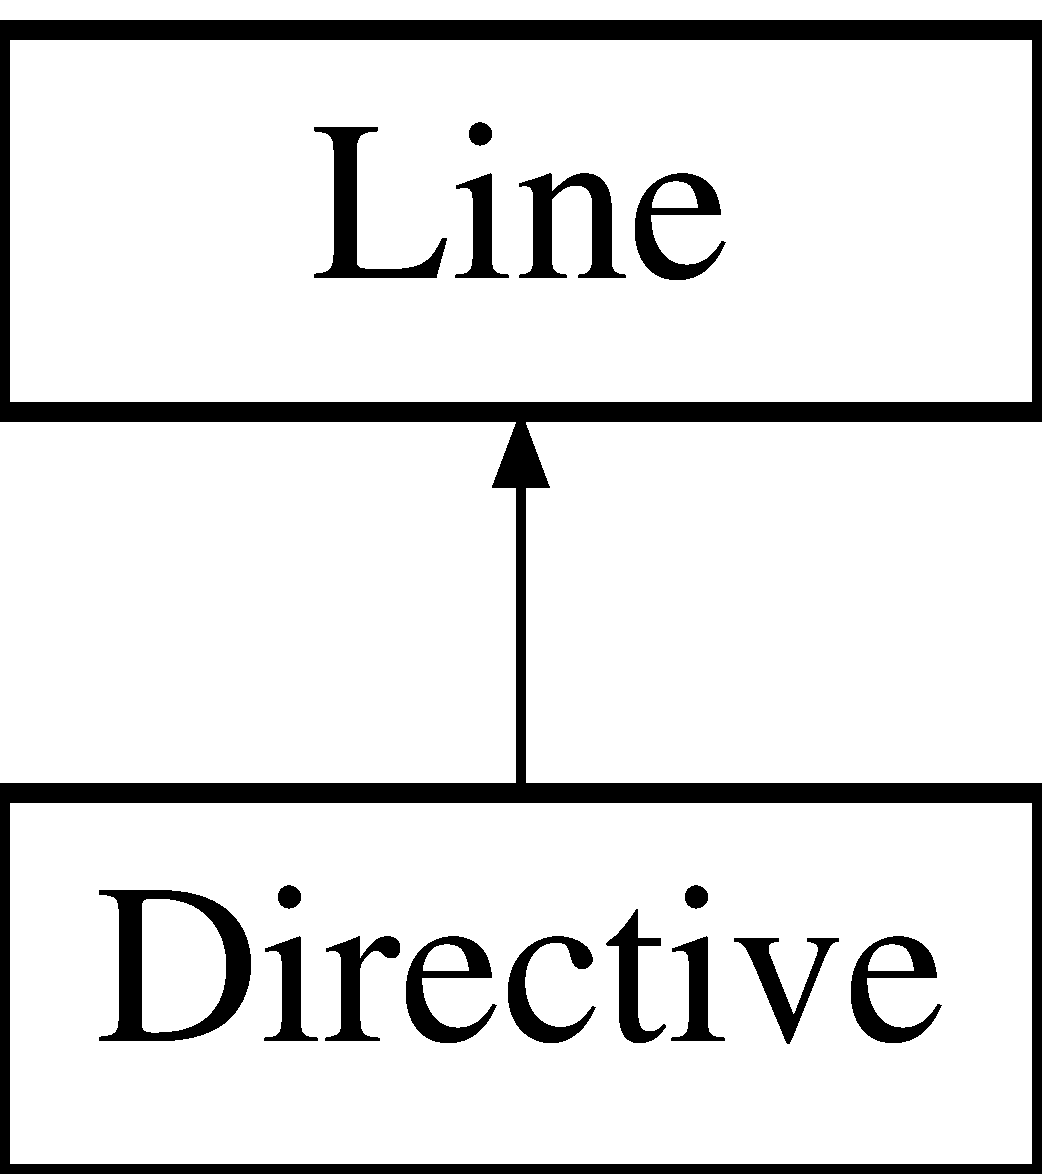
\includegraphics[height=2cm]{classDirective}
\end{center}
\end{figure}
\subsection*{Public Member Functions}
\begin{DoxyCompactItemize}
\item 
\hypertarget{classDirective_a7487120f679e1b4d01843ad6feac7e07}{
\hyperlink{classDirective_a7487120f679e1b4d01843ad6feac7e07}{Directive} (string)}
\label{classDirective_a7487120f679e1b4d01843ad6feac7e07}

\begin{DoxyCompactList}\small\item\em Constructor of the \hyperlink{classDirective}{Directive}. \item\end{DoxyCompactList}\item 
\hypertarget{classDirective_aa9a48f09b0472c835ffa366bcff74f51}{
virtual \hyperlink{classDirective_aa9a48f09b0472c835ffa366bcff74f51}{$\sim$Directive} ()}
\label{classDirective_aa9a48f09b0472c835ffa366bcff74f51}

\begin{DoxyCompactList}\small\item\em Destructor of the \hyperlink{classDirective}{Directive}. \item\end{DoxyCompactList}\item 
\hypertarget{classDirective_a900c72c92ff32e7a673030a07dae3176}{
virtual t\_\-Line \hyperlink{classDirective_a900c72c92ff32e7a673030a07dae3176}{typeLine} ()}
\label{classDirective_a900c72c92ff32e7a673030a07dae3176}

\begin{DoxyCompactList}\small\item\em get the type of the line \item\end{DoxyCompactList}\item 
\hypertarget{classDirective_a6eeb8fca1505c28a3f54864edb24457c}{
virtual string \hyperlink{classDirective_a6eeb8fca1505c28a3f54864edb24457c}{toString} ()}
\label{classDirective_a6eeb8fca1505c28a3f54864edb24457c}

\begin{DoxyCompactList}\small\item\em get the string of the \hyperlink{classDirective}{Directive} \item\end{DoxyCompactList}\item 
\hypertarget{classDirective_a13fa431d4e5957049311f8df5f50b383}{
virtual string \hyperlink{classDirective_a13fa431d4e5957049311f8df5f50b383}{getContent} ()}
\label{classDirective_a13fa431d4e5957049311f8df5f50b383}

\begin{DoxyCompactList}\small\item\em get the string of the \hyperlink{classDirective}{Directive} \item\end{DoxyCompactList}\item 
\hypertarget{classDirective_a015ce52f1282454208ebc613260a5c67}{
virtual void \hyperlink{classDirective_a015ce52f1282454208ebc613260a5c67}{setContent} (string)}
\label{classDirective_a015ce52f1282454208ebc613260a5c67}

\begin{DoxyCompactList}\small\item\em set the string of the \hyperlink{classDirective}{Directive} \item\end{DoxyCompactList}\item 
\hypertarget{classDirective_a5141831f1ebbe73fb15085790d1decfa}{
virtual bool \hyperlink{classDirective_a5141831f1ebbe73fb15085790d1decfa}{isFunction} ()}
\label{classDirective_a5141831f1ebbe73fb15085790d1decfa}

\begin{DoxyCompactList}\small\item\em return true if the directive indicate a function \item\end{DoxyCompactList}\item 
\hypertarget{classDirective_a97289e08e5fbfe822a15fd70fb1b48f3}{
virtual t\_\-Inst \hyperlink{classDirective_a97289e08e5fbfe822a15fd70fb1b48f3}{getType} ()}
\label{classDirective_a97289e08e5fbfe822a15fd70fb1b48f3}

\begin{DoxyCompactList}\small\item\em return the type of the instruction \item\end{DoxyCompactList}\end{DoxyCompactItemize}


\subsection{Detailed Description}
class representing an \hyperlink{classDirective}{Directive} herited by \hyperlink{classLine}{Line} 

The documentation for this class was generated from the following file:\begin{DoxyCompactItemize}
\item 
\hyperlink{Directive_8h}{Directive.h}\end{DoxyCompactItemize}

\hypertarget{classFunction}{
\section{Function Class Reference}
\label{classFunction}\index{Function@{Function}}
}


class representing a \hyperlink{classFunction}{Function} on a program  


{\ttfamily \#include $<$Function.h$>$}\subsection*{Public Member Functions}
\begin{DoxyCompactItemize}
\item 
\hypertarget{classFunction_ae206568fd4fd4c885e3ccff76345c4e6}{
\hyperlink{classFunction_ae206568fd4fd4c885e3ccff76345c4e6}{Function} ()}
\label{classFunction_ae206568fd4fd4c885e3ccff76345c4e6}

\begin{DoxyCompactList}\small\item\em Constructor of a function. \item\end{DoxyCompactList}\item 
\hypertarget{classFunction_a3b03f7cf0b75d16edebdda1dee1db6fd}{
\hyperlink{classFunction_a3b03f7cf0b75d16edebdda1dee1db6fd}{$\sim$Function} ()}
\label{classFunction_a3b03f7cf0b75d16edebdda1dee1db6fd}

\begin{DoxyCompactList}\small\item\em Destructor of a function. \item\end{DoxyCompactList}\item 
\hypertarget{classFunction_a39d6ea7220c44d9bb67e2a644ed679d1}{
void \hyperlink{classFunction_a39d6ea7220c44d9bb67e2a644ed679d1}{set\_\-head} (\hyperlink{classNode}{Node} $\ast$)}
\label{classFunction_a39d6ea7220c44d9bb67e2a644ed679d1}

\begin{DoxyCompactList}\small\item\em setter of the head of the function \item\end{DoxyCompactList}\item 
\hypertarget{classFunction_a741002f6a0c79c49afe9cf7c8628159d}{
void \hyperlink{classFunction_a741002f6a0c79c49afe9cf7c8628159d}{set\_\-end} (\hyperlink{classNode}{Node} $\ast$)}
\label{classFunction_a741002f6a0c79c49afe9cf7c8628159d}

\begin{DoxyCompactList}\small\item\em setter of the end of the function \item\end{DoxyCompactList}\item 
\hypertarget{classFunction_ad166c144498bcd0c82efd71a9ce38fd5}{
\hyperlink{classNode}{Node} $\ast$ \hyperlink{classFunction_ad166c144498bcd0c82efd71a9ce38fd5}{get\_\-head} ()}
\label{classFunction_ad166c144498bcd0c82efd71a9ce38fd5}

\begin{DoxyCompactList}\small\item\em get the head of the function \item\end{DoxyCompactList}\item 
\hypertarget{classFunction_a57e6d0f497252ac29597e3b65d9f856a}{
\hyperlink{classNode}{Node} $\ast$ \hyperlink{classFunction_a57e6d0f497252ac29597e3b65d9f856a}{get\_\-end} ()}
\label{classFunction_a57e6d0f497252ac29597e3b65d9f856a}

\begin{DoxyCompactList}\small\item\em get the end of the function \item\end{DoxyCompactList}\item 
\hypertarget{classFunction_ade8a6050da83010be473a6581d65a3ce}{
void \hyperlink{classFunction_ade8a6050da83010be473a6581d65a3ce}{display} ()}
\label{classFunction_ade8a6050da83010be473a6581d65a3ce}

\begin{DoxyCompactList}\small\item\em display the function \item\end{DoxyCompactList}\item 
\hypertarget{classFunction_a0b62379b4e18c9440963b54d2e8991b0}{
int \hyperlink{classFunction_a0b62379b4e18c9440963b54d2e8991b0}{size} ()}
\label{classFunction_a0b62379b4e18c9440963b54d2e8991b0}

\begin{DoxyCompactList}\small\item\em get the size of the function \item\end{DoxyCompactList}\item 
\hypertarget{classFunction_acd08be840c48abd3c0c0c20ca4b5192a}{
void \hyperlink{classFunction_acd08be840c48abd3c0c0c20ca4b5192a}{restitution} (string const)}
\label{classFunction_acd08be840c48abd3c0c0c20ca4b5192a}

\begin{DoxyCompactList}\small\item\em restitute the function in a file \item\end{DoxyCompactList}\item 
\hypertarget{classFunction_a6094f123294ccbb891fa4145fd5b1b0a}{
void \hyperlink{classFunction_a6094f123294ccbb891fa4145fd5b1b0a}{comput\_\-basic\_\-block} ()}
\label{classFunction_a6094f123294ccbb891fa4145fd5b1b0a}

\begin{DoxyCompactList}\small\item\em Calculate the basics bolck of the function. \item\end{DoxyCompactList}\item 
\hypertarget{classFunction_a4ddde4ac1ff488dfcbfcaee71f727a48}{
int \hyperlink{classFunction_a4ddde4ac1ff488dfcbfcaee71f727a48}{nbr\_\-BB} ()}
\label{classFunction_a4ddde4ac1ff488dfcbfcaee71f727a48}

\begin{DoxyCompactList}\small\item\em get the number of Basic block in the function \item\end{DoxyCompactList}\item 
\hypertarget{classFunction_ad145d230633705dc2a51789d11fe8649}{
\hyperlink{classBasic__block}{Basic\_\-block} \hyperlink{classFunction_ad145d230633705dc2a51789d11fe8649}{get\_\-BB} (int)}
\label{classFunction_ad145d230633705dc2a51789d11fe8649}

\begin{DoxyCompactList}\small\item\em get the Basic Block in the list \item\end{DoxyCompactList}\end{DoxyCompactItemize}


\subsection{Detailed Description}
class representing a \hyperlink{classFunction}{Function} on a program 

The documentation for this class was generated from the following file:\begin{DoxyCompactItemize}
\item 
\hyperlink{Function_8h}{Function.h}\end{DoxyCompactItemize}

\hypertarget{classInstruction}{
\section{Instruction Class Reference}
\label{classInstruction}\index{Instruction@{Instruction}}
}


class representing an instruction which herited by \hyperlink{classLine}{Line}  


{\ttfamily \#include $<$Instruction.h$>$}Inheritance diagram for Instruction::\begin{figure}[H]
\begin{center}
\leavevmode
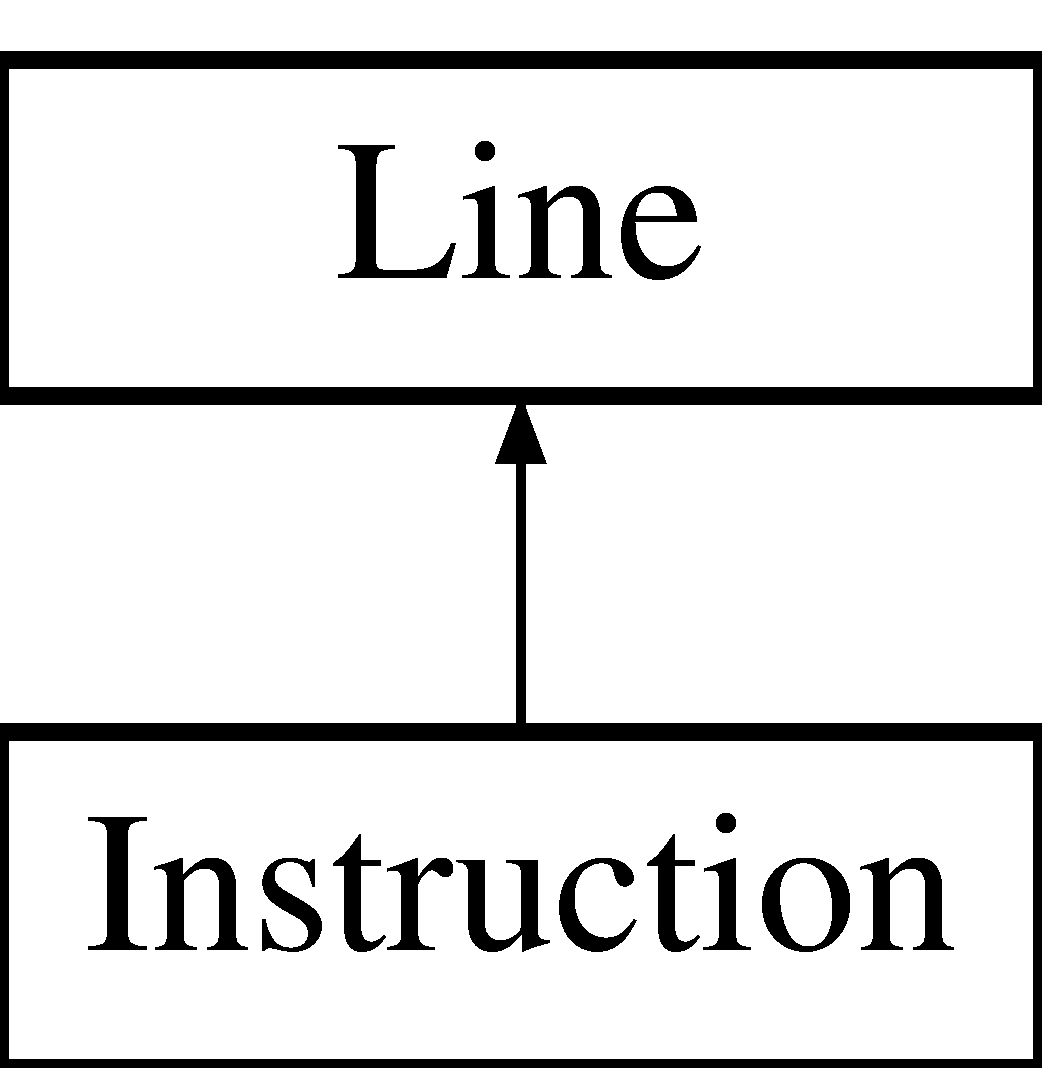
\includegraphics[height=2cm]{classInstruction}
\end{center}
\end{figure}
\subsection*{Public Member Functions}
\begin{DoxyCompactItemize}
\item 
\hypertarget{classInstruction_ae0035f2c32d1a7219ef303014473072f}{
\hyperlink{classInstruction_ae0035f2c32d1a7219ef303014473072f}{Instruction} (string, t\_\-Operator, t\_\-Format, t\_\-Inst, \hyperlink{classOperand}{Operand} $\ast$, \hyperlink{classOperand}{Operand} $\ast$, \hyperlink{classOperand}{Operand} $\ast$, int)}
\label{classInstruction_ae0035f2c32d1a7219ef303014473072f}

\begin{DoxyCompactList}\small\item\em Constructor of the class instruction. \item\end{DoxyCompactList}\item 
\hypertarget{classInstruction_a2f1ed1606d4090b8a4c255e3af9e34c8}{
\hyperlink{classInstruction_a2f1ed1606d4090b8a4c255e3af9e34c8}{Instruction} (t\_\-Operator, \hyperlink{classOperand}{Operand} $\ast$, \hyperlink{classOperand}{Operand} $\ast$, \hyperlink{classOperand}{Operand} $\ast$)}
\label{classInstruction_a2f1ed1606d4090b8a4c255e3af9e34c8}

\begin{DoxyCompactList}\small\item\em Constructor with 3 Operands of the class instruction. \item\end{DoxyCompactList}\item 
\hypertarget{classInstruction_a0b1ed4432c9c5823ee9e522c7d11bb5f}{
\hyperlink{classInstruction_a0b1ed4432c9c5823ee9e522c7d11bb5f}{Instruction} (t\_\-Operator, \hyperlink{classOperand}{Operand} $\ast$, \hyperlink{classOperand}{Operand} $\ast$)}
\label{classInstruction_a0b1ed4432c9c5823ee9e522c7d11bb5f}

\begin{DoxyCompactList}\small\item\em Constructor with 2 Operands of the class instruction. \item\end{DoxyCompactList}\item 
\hypertarget{classInstruction_a6ae2a4dd83500f9d538a653823161b1c}{
\hyperlink{classInstruction_a6ae2a4dd83500f9d538a653823161b1c}{Instruction} (t\_\-Operator, \hyperlink{classOperand}{Operand} $\ast$)}
\label{classInstruction_a6ae2a4dd83500f9d538a653823161b1c}

\begin{DoxyCompactList}\small\item\em Constructor with 1 \hyperlink{classOperand}{Operand} of the class instruction. \item\end{DoxyCompactList}\item 
\hypertarget{classInstruction_ab2d989cc18e9bf0eeee194a7614514fa}{
\hyperlink{classInstruction_ab2d989cc18e9bf0eeee194a7614514fa}{Instruction} (t\_\-Operator)}
\label{classInstruction_ab2d989cc18e9bf0eeee194a7614514fa}

\begin{DoxyCompactList}\small\item\em Constructor without Operands of the class instruction. \item\end{DoxyCompactList}\item 
\hypertarget{classInstruction_a3f1031e811b710787678f8faf8cc9672}{
virtual \hyperlink{classInstruction_a3f1031e811b710787678f8faf8cc9672}{$\sim$Instruction} ()}
\label{classInstruction_a3f1031e811b710787678f8faf8cc9672}

\begin{DoxyCompactList}\small\item\em Destructor of the class instruction. \item\end{DoxyCompactList}\item 
\hypertarget{classInstruction_a04e2ccada02259b6308917df6cefd06d}{
\hyperlink{classOperand}{Operand} $\ast$ \hyperlink{classInstruction_a04e2ccada02259b6308917df6cefd06d}{getOp1} ()}
\label{classInstruction_a04e2ccada02259b6308917df6cefd06d}

\begin{DoxyCompactList}\small\item\em Get the first operand value accessor of the operand. \item\end{DoxyCompactList}\item 
\hypertarget{classInstruction_ad98f97337a6a2a1bfe344bd79fe54559}{
void \hyperlink{classInstruction_ad98f97337a6a2a1bfe344bd79fe54559}{setOp1} (\hyperlink{classOperand}{Operand} $\ast$o)}
\label{classInstruction_ad98f97337a6a2a1bfe344bd79fe54559}

\begin{DoxyCompactList}\small\item\em set the first operand value setter of the operand \item\end{DoxyCompactList}\item 
\hypertarget{classInstruction_a51c7c00f098ae7b0e824f77d091ea584}{
\hyperlink{classOperand}{Operand} $\ast$ \hyperlink{classInstruction_a51c7c00f098ae7b0e824f77d091ea584}{getOp2} ()}
\label{classInstruction_a51c7c00f098ae7b0e824f77d091ea584}

\begin{DoxyCompactList}\small\item\em Get the second operand value accessor of the operand. \item\end{DoxyCompactList}\item 
\hypertarget{classInstruction_a33a107262438a4f63730c82a1f30300e}{
void \hyperlink{classInstruction_a33a107262438a4f63730c82a1f30300e}{setOp2} (\hyperlink{classOperand}{Operand} $\ast$o)}
\label{classInstruction_a33a107262438a4f63730c82a1f30300e}

\begin{DoxyCompactList}\small\item\em set the second operand value setter of the operand \item\end{DoxyCompactList}\item 
\hypertarget{classInstruction_af871b07a0cc69f1c8bdcff9b7ee50ba3}{
\hyperlink{classOperand}{Operand} $\ast$ \hyperlink{classInstruction_af871b07a0cc69f1c8bdcff9b7ee50ba3}{getOp3} ()}
\label{classInstruction_af871b07a0cc69f1c8bdcff9b7ee50ba3}

\begin{DoxyCompactList}\small\item\em Get the third operand value accessor of the operand. \item\end{DoxyCompactList}\item 
\hypertarget{classInstruction_a29ee9d49576d6403fd81ce57967278ef}{
void \hyperlink{classInstruction_a29ee9d49576d6403fd81ce57967278ef}{setOp3} (\hyperlink{classOperand}{Operand} $\ast$o)}
\label{classInstruction_a29ee9d49576d6403fd81ce57967278ef}

\begin{DoxyCompactList}\small\item\em set the third operand value setter of the operand \item\end{DoxyCompactList}\item 
\hypertarget{classInstruction_a973185cd0d1e01d62115a8b1da956f9f}{
t\_\-Operator \hyperlink{classInstruction_a973185cd0d1e01d62115a8b1da956f9f}{getOPcode} ()}
\label{classInstruction_a973185cd0d1e01d62115a8b1da956f9f}

\begin{DoxyCompactList}\small\item\em get the Opcode value accessor of the opcode \item\end{DoxyCompactList}\item 
\hypertarget{classInstruction_af372e543adb180ce7c9433e3b0d3cd1f}{
string \hyperlink{classInstruction_af372e543adb180ce7c9433e3b0d3cd1f}{stringOPcode} ()}
\label{classInstruction_af372e543adb180ce7c9433e3b0d3cd1f}

\begin{DoxyCompactList}\small\item\em get the string Opcode value accessor of the string opcode \item\end{DoxyCompactList}\item 
\hypertarget{classInstruction_af679b991cc01ab560863e6f428703a49}{
void \hyperlink{classInstruction_af679b991cc01ab560863e6f428703a49}{setOPcode} (t\_\-Operator newop)}
\label{classInstruction_af679b991cc01ab560863e6f428703a49}

\begin{DoxyCompactList}\small\item\em set the opcode value setter of the opcode \item\end{DoxyCompactList}\item 
\hypertarget{classInstruction_a001e765d27e7d59bbca718284ab0a2e3}{
t\_\-Format \hyperlink{classInstruction_a001e765d27e7d59bbca718284ab0a2e3}{getFormat} ()}
\label{classInstruction_a001e765d27e7d59bbca718284ab0a2e3}

\begin{DoxyCompactList}\small\item\em get the format of the \hyperlink{classInstruction}{Instruction} accessor of the format \item\end{DoxyCompactList}\item 
\hypertarget{classInstruction_aeef5ced47cdd5477ba0809bf372b8a72}{
virtual t\_\-Inst \hyperlink{classInstruction_aeef5ced47cdd5477ba0809bf372b8a72}{getType} ()}
\label{classInstruction_aeef5ced47cdd5477ba0809bf372b8a72}

\begin{DoxyCompactList}\small\item\em get the Type of the \hyperlink{classInstruction}{Instruction} accessor of the Type \item\end{DoxyCompactList}\item 
\hypertarget{classInstruction_ad14cb84b8fa70f3e47271d72f7c640a4}{
virtual t\_\-Line \hyperlink{classInstruction_ad14cb84b8fa70f3e47271d72f7c640a4}{typeLine} ()}
\label{classInstruction_ad14cb84b8fa70f3e47271d72f7c640a4}

\begin{DoxyCompactList}\small\item\em get the type of the line \item\end{DoxyCompactList}\item 
\hypertarget{classInstruction_ad892da43543a6b385962a4992fbc76b5}{
virtual string \hyperlink{classInstruction_ad892da43543a6b385962a4992fbc76b5}{toString} ()}
\label{classInstruction_ad892da43543a6b385962a4992fbc76b5}

\begin{DoxyCompactList}\small\item\em get the name string instruction \item\end{DoxyCompactList}\item 
\hypertarget{classInstruction_a24f58a3b18a0c9d66d90ed367a3af748}{
virtual string \hyperlink{classInstruction_a24f58a3b18a0c9d66d90ed367a3af748}{getContent} ()}
\label{classInstruction_a24f58a3b18a0c9d66d90ed367a3af748}

\begin{DoxyCompactList}\small\item\em get the string of the instruction \item\end{DoxyCompactList}\item 
\hypertarget{classInstruction_adb8a823e8a4b3ffa6a7645ec2fefe07c}{
virtual void \hyperlink{classInstruction_adb8a823e8a4b3ffa6a7645ec2fefe07c}{setContent} (string)}
\label{classInstruction_adb8a823e8a4b3ffa6a7645ec2fefe07c}

\begin{DoxyCompactList}\small\item\em set the string of the instruction \item\end{DoxyCompactList}\item 
\hypertarget{classInstruction_aed69e1f72d4ad277672b6b2ff0c2be10}{
string \hyperlink{classInstruction_aed69e1f72d4ad277672b6b2ff0c2be10}{stringForm} ()}
\label{classInstruction_aed69e1f72d4ad277672b6b2ff0c2be10}

\begin{DoxyCompactList}\small\item\em set the string format \item\end{DoxyCompactList}\item 
\hypertarget{classInstruction_a030d0966d0bfd352f21a6ddaa1ab95bc}{
string \hyperlink{classInstruction_a030d0966d0bfd352f21a6ddaa1ab95bc}{stringType} ()}
\label{classInstruction_a030d0966d0bfd352f21a6ddaa1ab95bc}

\begin{DoxyCompactList}\small\item\em set the string Type of instruction \item\end{DoxyCompactList}\item 
t\_\-Dep \hyperlink{classInstruction_a7e93717c1e9df6fed09105accb6c728c}{is\_\-dependant} (\hyperlink{classInstruction}{Instruction} i2)
\begin{DoxyCompactList}\small\item\em get the dependance between the current instruction and i2 \item\end{DoxyCompactList}\item 
bool \hyperlink{classInstruction_a757d13233614f3b81f340275e0ac03fc}{is\_\-dep\_\-RAW} (\hyperlink{classInstruction}{Instruction} i2)
\begin{DoxyCompactList}\small\item\em get the information if there is dependance RAW between the current instruction and i2 \item\end{DoxyCompactList}\item 
bool \hyperlink{classInstruction_a22c2bbac305649d7f0ec17a04ef217fc}{is\_\-dep\_\-WAR} (\hyperlink{classInstruction}{Instruction} i2)
\begin{DoxyCompactList}\small\item\em get the information if there is dependance WAR between the current instruction and i2 \item\end{DoxyCompactList}\item 
bool \hyperlink{classInstruction_a6fd4dd46f540f0674486d559c1fbcd57}{is\_\-dep\_\-WAW} (\hyperlink{classInstruction}{Instruction} i2)
\begin{DoxyCompactList}\small\item\em get the information if there is dependance WAW between the current instruction and i2 \item\end{DoxyCompactList}\item 
int \hyperlink{classInstruction_a3278668f293095ccb1565f36894a117e}{getNumberOper} ()
\begin{DoxyCompactList}\small\item\em get the number of operand \item\end{DoxyCompactList}\item 
\hypertarget{classInstruction_a748889b83c25f1e791fbbc44d2414f99}{
void \hyperlink{classInstruction_a748889b83c25f1e791fbbc44d2414f99}{setNumberOper} (int)}
\label{classInstruction_a748889b83c25f1e791fbbc44d2414f99}

\begin{DoxyCompactList}\small\item\em set the number of operand \item\end{DoxyCompactList}\item 
\hypertarget{classInstruction_ac7d969cbfe439058d54a78f924e46b8e}{
virtual bool \hyperlink{classInstruction_ac7d969cbfe439058d54a78f924e46b8e}{isFunction} ()}
\label{classInstruction_ac7d969cbfe439058d54a78f924e46b8e}

\begin{DoxyCompactList}\small\item\em return true if the directive indicate a function \item\end{DoxyCompactList}\item 
\hypertarget{classInstruction_ab479411998d84d1fab040fe9d09e3ea3}{
\hyperlink{classOperand}{Operand} $\ast$ \hyperlink{classInstruction_ab479411998d84d1fab040fe9d09e3ea3}{getRegDst} ()}
\label{classInstruction_ab479411998d84d1fab040fe9d09e3ea3}

\begin{DoxyCompactList}\small\item\em get the regiter destination of the instruction \item\end{DoxyCompactList}\item 
\hypertarget{classInstruction_a71763d6a2b2a1d64b3115ca78bce736b}{
\hyperlink{classOperand}{Operand} $\ast$ \hyperlink{classInstruction_a71763d6a2b2a1d64b3115ca78bce736b}{getRegSrc1} ()}
\label{classInstruction_a71763d6a2b2a1d64b3115ca78bce736b}

\begin{DoxyCompactList}\small\item\em get the first register source of the instruction \item\end{DoxyCompactList}\item 
\hypertarget{classInstruction_ae896b626e81e6213db9c23147b50d960}{
\hyperlink{classOperand}{Operand} $\ast$ \hyperlink{classInstruction_ae896b626e81e6213db9c23147b50d960}{getRegSrc2} ()}
\label{classInstruction_ae896b626e81e6213db9c23147b50d960}

\begin{DoxyCompactList}\small\item\em get the second register source of the instruction \item\end{DoxyCompactList}\end{DoxyCompactItemize}


\subsection{Detailed Description}
class representing an instruction which herited by \hyperlink{classLine}{Line} 

\subsection{Member Function Documentation}
\hypertarget{classInstruction_a3278668f293095ccb1565f36894a117e}{
\index{Instruction@{Instruction}!getNumberOper@{getNumberOper}}
\index{getNumberOper@{getNumberOper}!Instruction@{Instruction}}
\subsubsection[{getNumberOper}]{\setlength{\rightskip}{0pt plus 5cm}int Instruction::getNumberOper ()}}
\label{classInstruction_a3278668f293095ccb1565f36894a117e}


get the number of operand \begin{DoxyReturn}{Returns}
return the number of operand 
\end{DoxyReturn}
\hypertarget{classInstruction_a757d13233614f3b81f340275e0ac03fc}{
\index{Instruction@{Instruction}!is\_\-dep\_\-RAW@{is\_\-dep\_\-RAW}}
\index{is\_\-dep\_\-RAW@{is\_\-dep\_\-RAW}!Instruction@{Instruction}}
\subsubsection[{is\_\-dep\_\-RAW}]{\setlength{\rightskip}{0pt plus 5cm}bool Instruction::is\_\-dep\_\-RAW ({\bf Instruction} {\em i2})}}
\label{classInstruction_a757d13233614f3b81f340275e0ac03fc}


get the information if there is dependance RAW between the current instruction and i2 \begin{DoxyReturn}{Returns}
return true if there is a RAW dependance 
\end{DoxyReturn}
\hypertarget{classInstruction_a22c2bbac305649d7f0ec17a04ef217fc}{
\index{Instruction@{Instruction}!is\_\-dep\_\-WAR@{is\_\-dep\_\-WAR}}
\index{is\_\-dep\_\-WAR@{is\_\-dep\_\-WAR}!Instruction@{Instruction}}
\subsubsection[{is\_\-dep\_\-WAR}]{\setlength{\rightskip}{0pt plus 5cm}bool Instruction::is\_\-dep\_\-WAR ({\bf Instruction} {\em i2})}}
\label{classInstruction_a22c2bbac305649d7f0ec17a04ef217fc}


get the information if there is dependance WAR between the current instruction and i2 \begin{DoxyReturn}{Returns}
return true if there is a WAR dependance 
\end{DoxyReturn}
\hypertarget{classInstruction_a6fd4dd46f540f0674486d559c1fbcd57}{
\index{Instruction@{Instruction}!is\_\-dep\_\-WAW@{is\_\-dep\_\-WAW}}
\index{is\_\-dep\_\-WAW@{is\_\-dep\_\-WAW}!Instruction@{Instruction}}
\subsubsection[{is\_\-dep\_\-WAW}]{\setlength{\rightskip}{0pt plus 5cm}bool Instruction::is\_\-dep\_\-WAW ({\bf Instruction} {\em i2})}}
\label{classInstruction_a6fd4dd46f540f0674486d559c1fbcd57}


get the information if there is dependance WAW between the current instruction and i2 \begin{DoxyReturn}{Returns}
return true if there is a WAW dependance 
\end{DoxyReturn}
\hypertarget{classInstruction_a7e93717c1e9df6fed09105accb6c728c}{
\index{Instruction@{Instruction}!is\_\-dependant@{is\_\-dependant}}
\index{is\_\-dependant@{is\_\-dependant}!Instruction@{Instruction}}
\subsubsection[{is\_\-dependant}]{\setlength{\rightskip}{0pt plus 5cm}t\_\-Dep Instruction::is\_\-dependant ({\bf Instruction} {\em i2})}}
\label{classInstruction_a7e93717c1e9df6fed09105accb6c728c}


get the dependance between the current instruction and i2 \begin{DoxyReturn}{Returns}
return \char`\"{}RAW\char`\"{}, \char`\"{}WAR\char`\"{}, \char`\"{}WAW\char`\"{} or \char`\"{}not dependant\char`\"{} in format enum 
\end{DoxyReturn}


The documentation for this class was generated from the following file:\begin{DoxyCompactItemize}
\item 
\hyperlink{Instruction_8h}{Instruction.h}\end{DoxyCompactItemize}

\hypertarget{classLabel}{
\section{Label Class Reference}
\label{classLabel}\index{Label@{Label}}
}


class representing an \hyperlink{classLabel}{Label} herited by \hyperlink{classLine}{Line}  


{\ttfamily \#include $<$Label.h$>$}Inheritance diagram for Label::\begin{figure}[H]
\begin{center}
\leavevmode
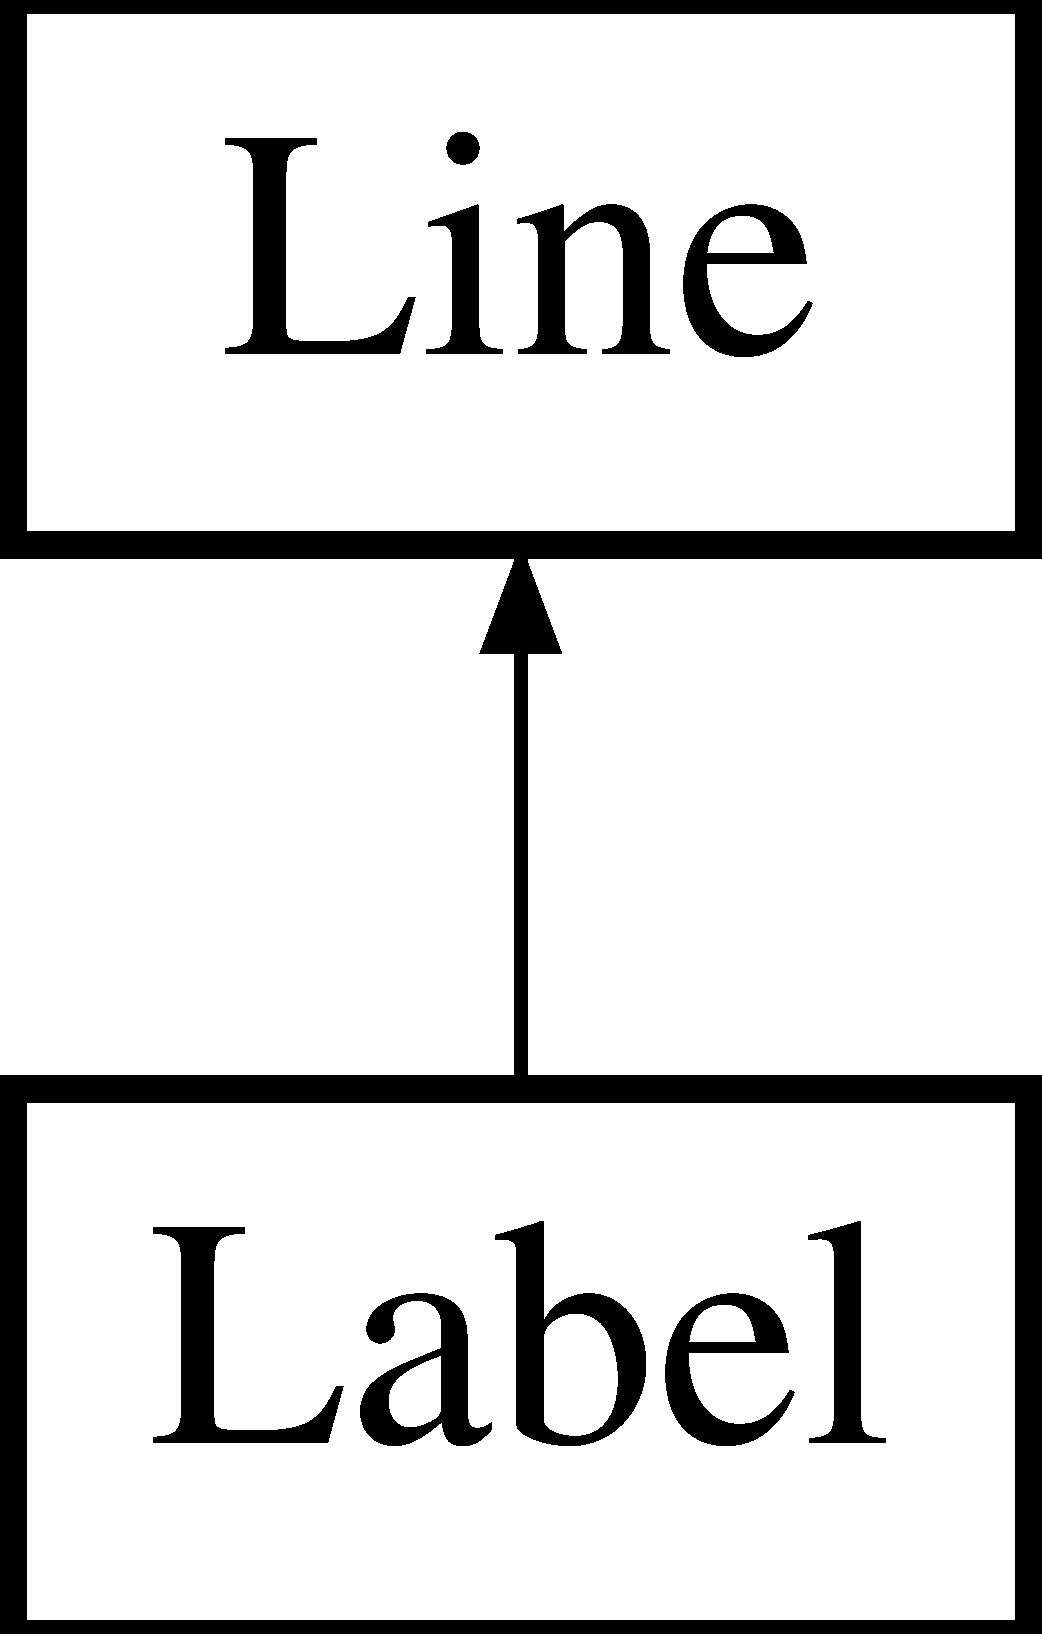
\includegraphics[height=2cm]{classLabel}
\end{center}
\end{figure}
\subsection*{Public Member Functions}
\begin{DoxyCompactItemize}
\item 
\hypertarget{classLabel_a48e774efc0e6e5cd0bf63a94527add17}{
\hyperlink{classLabel_a48e774efc0e6e5cd0bf63a94527add17}{Label} (string)}
\label{classLabel_a48e774efc0e6e5cd0bf63a94527add17}

\begin{DoxyCompactList}\small\item\em Constructor of the \hyperlink{classLabel}{Label}. \item\end{DoxyCompactList}\item 
\hypertarget{classLabel_ae0405d591a2ff63c03b104435e2a3066}{
virtual \hyperlink{classLabel_ae0405d591a2ff63c03b104435e2a3066}{$\sim$Label} ()}
\label{classLabel_ae0405d591a2ff63c03b104435e2a3066}

\begin{DoxyCompactList}\small\item\em Destructor of the \hyperlink{classLabel}{Label}. \item\end{DoxyCompactList}\item 
\hypertarget{classLabel_a83977f94c80e2a8fc38271ff6ffb2696}{
virtual t\_\-Line \hyperlink{classLabel_a83977f94c80e2a8fc38271ff6ffb2696}{typeLine} ()}
\label{classLabel_a83977f94c80e2a8fc38271ff6ffb2696}

\begin{DoxyCompactList}\small\item\em get the type of the line \item\end{DoxyCompactList}\item 
\hypertarget{classLabel_a2bf18281612263a76e02a9d1f3e3a009}{
virtual string \hyperlink{classLabel_a2bf18281612263a76e02a9d1f3e3a009}{toString} ()}
\label{classLabel_a2bf18281612263a76e02a9d1f3e3a009}

\begin{DoxyCompactList}\small\item\em get the string of \hyperlink{classLabel}{Label} \item\end{DoxyCompactList}\item 
\hypertarget{classLabel_a552b9c44da6aee5c68996e466391f04a}{
virtual string \hyperlink{classLabel_a552b9c44da6aee5c68996e466391f04a}{getContent} ()}
\label{classLabel_a552b9c44da6aee5c68996e466391f04a}

\begin{DoxyCompactList}\small\item\em get the string of the \hyperlink{classLabel}{Label} \item\end{DoxyCompactList}\item 
\hypertarget{classLabel_a80c83b9767d0b3116d603c79973ffb6b}{
virtual void \hyperlink{classLabel_a80c83b9767d0b3116d603c79973ffb6b}{setContent} (string)}
\label{classLabel_a80c83b9767d0b3116d603c79973ffb6b}

\begin{DoxyCompactList}\small\item\em set the string of the \hyperlink{classLabel}{Label} \item\end{DoxyCompactList}\item 
\hypertarget{classLabel_a891d14c5e6d110964ba55a3ecddc0999}{
virtual bool \hyperlink{classLabel_a891d14c5e6d110964ba55a3ecddc0999}{isFunction} ()}
\label{classLabel_a891d14c5e6d110964ba55a3ecddc0999}

\begin{DoxyCompactList}\small\item\em return true if the directive indicate a function \item\end{DoxyCompactList}\item 
\hypertarget{classLabel_ae988d31522bce75a19fabca6e4aaedc9}{
virtual t\_\-Inst \hyperlink{classLabel_ae988d31522bce75a19fabca6e4aaedc9}{getType} ()}
\label{classLabel_ae988d31522bce75a19fabca6e4aaedc9}

\begin{DoxyCompactList}\small\item\em return the type of the instruction \item\end{DoxyCompactList}\end{DoxyCompactItemize}


\subsection{Detailed Description}
class representing an \hyperlink{classLabel}{Label} herited by \hyperlink{classLine}{Line} 

The documentation for this class was generated from the following file:\begin{DoxyCompactItemize}
\item 
\hyperlink{Label_8h}{Label.h}\end{DoxyCompactItemize}

\hypertarget{classLine}{
\section{Line Class Reference}
\label{classLine}\index{Line@{Line}}
}


Abstract class representing an \hyperlink{classLine}{Line}.  


{\ttfamily \#include $<$Line.h$>$}Inheritance diagram for Line::\begin{figure}[H]
\begin{center}
\leavevmode
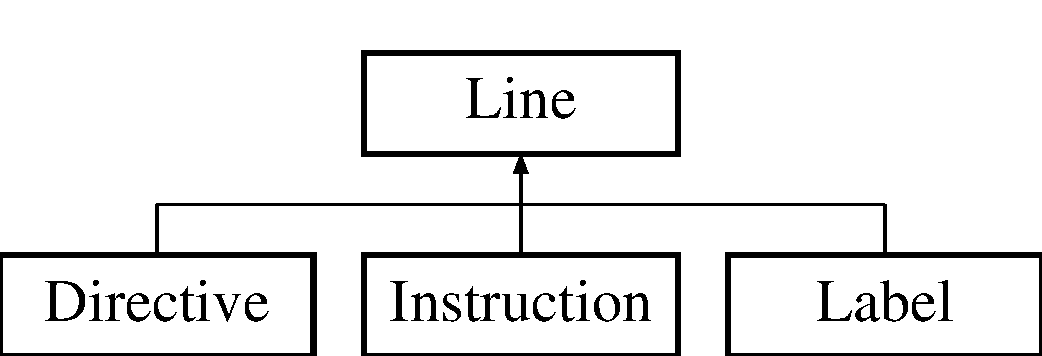
\includegraphics[height=2cm]{classLine}
\end{center}
\end{figure}
\subsection*{Public Member Functions}
\begin{DoxyCompactItemize}
\item 
\hypertarget{classLine_a4a95bafcefa28672b3999deb011b9e50}{
virtual \hyperlink{classLine_a4a95bafcefa28672b3999deb011b9e50}{$\sim$Line} ()}
\label{classLine_a4a95bafcefa28672b3999deb011b9e50}

\begin{DoxyCompactList}\small\item\em Virtual destructor. \item\end{DoxyCompactList}\item 
\hypertarget{classLine_a5d33e3b08ba3367ec5e685af342b2268}{
virtual string \hyperlink{classLine_a5d33e3b08ba3367ec5e685af342b2268}{getContent} ()=0}
\label{classLine_a5d33e3b08ba3367ec5e685af342b2268}

\begin{DoxyCompactList}\small\item\em get the string of the line virtual getter \item\end{DoxyCompactList}\item 
\hypertarget{classLine_a13407b1549d23dc3a863c063bd96df05}{
virtual void \hyperlink{classLine_a13407b1549d23dc3a863c063bd96df05}{setContent} (string)=0}
\label{classLine_a13407b1549d23dc3a863c063bd96df05}

\begin{DoxyCompactList}\small\item\em set the string of the line virtual setter \item\end{DoxyCompactList}\item 
\hypertarget{classLine_aafc83899e2d7208eef2f53702c86d539}{
virtual t\_\-Line \hyperlink{classLine_aafc83899e2d7208eef2f53702c86d539}{typeLine} ()=0}
\label{classLine_aafc83899e2d7208eef2f53702c86d539}

\begin{DoxyCompactList}\small\item\em get the type of the line virtual accessor of the type \item\end{DoxyCompactList}\item 
virtual string \hyperlink{classLine_a73f822ce0aa9e95bc8fb2caf1a69b245}{toString} ()=0
\begin{DoxyCompactList}\small\item\em get the name string accessor of the type line \item\end{DoxyCompactList}\item 
\hypertarget{classLine_a0bee811e73e0c4f55ef1e12325490478}{
virtual bool \hyperlink{classLine_a0bee811e73e0c4f55ef1e12325490478}{isFunction} ()=0}
\label{classLine_a0bee811e73e0c4f55ef1e12325490478}

\begin{DoxyCompactList}\small\item\em return true if the directive indicate a function \item\end{DoxyCompactList}\item 
\hypertarget{classLine_a8673983ef23628b80ea1e4d0a14ce53e}{
virtual t\_\-Inst \hyperlink{classLine_a8673983ef23628b80ea1e4d0a14ce53e}{getType} ()=0}
\label{classLine_a8673983ef23628b80ea1e4d0a14ce53e}

\begin{DoxyCompactList}\small\item\em return the type of the instruction \item\end{DoxyCompactList}\end{DoxyCompactItemize}
\subsection*{Protected Attributes}
\begin{DoxyCompactItemize}
\item 
\hypertarget{classLine_a41059923f5c8e5a0f4f44d84bd8762aa}{
string {\bfseries \_\-line}}
\label{classLine_a41059923f5c8e5a0f4f44d84bd8762aa}

\end{DoxyCompactItemize}


\subsection{Detailed Description}
Abstract class representing an \hyperlink{classLine}{Line}. 

\subsection{Member Function Documentation}
\hypertarget{classLine_a73f822ce0aa9e95bc8fb2caf1a69b245}{
\index{Line@{Line}!toString@{toString}}
\index{toString@{toString}!Line@{Line}}
\subsubsection[{toString}]{\setlength{\rightskip}{0pt plus 5cm}virtual string Line::toString ()\hspace{0.3cm}{\ttfamily  \mbox{[}pure virtual\mbox{]}}}}
\label{classLine_a73f822ce0aa9e95bc8fb2caf1a69b245}


get the name string accessor of the type line 

Implemented in \hyperlink{classDirective_a6eeb8fca1505c28a3f54864edb24457c}{Directive}, \hyperlink{classInstruction_ad892da43543a6b385962a4992fbc76b5}{Instruction}, and \hyperlink{classLabel_a2bf18281612263a76e02a9d1f3e3a009}{Label}.

The documentation for this class was generated from the following file:\begin{DoxyCompactItemize}
\item 
\hyperlink{Line_8h}{Line.h}\end{DoxyCompactItemize}

\hypertarget{classNode}{
\section{Node Class Reference}
\label{classNode}\index{Node@{Node}}
}


class representing a \hyperlink{classNode}{Node} in list  


{\ttfamily \#include $<$Node.h$>$}\subsection*{Public Member Functions}
\begin{DoxyCompactItemize}
\item 
\hypertarget{classNode_a38b4c6850bd8b7f57986ab2131b09918}{
\hyperlink{classNode_a38b4c6850bd8b7f57986ab2131b09918}{Node} (\hyperlink{classLine}{Line} $\ast$content)}
\label{classNode_a38b4c6850bd8b7f57986ab2131b09918}

\begin{DoxyCompactList}\small\item\em \hyperlink{classNode}{Node} constructor. \item\end{DoxyCompactList}\item 
\hypertarget{classNode_aa0840c3cb5c7159be6d992adecd2097c}{
\hyperlink{classNode_aa0840c3cb5c7159be6d992adecd2097c}{$\sim$Node} ()}
\label{classNode_aa0840c3cb5c7159be6d992adecd2097c}

\begin{DoxyCompactList}\small\item\em \hyperlink{classNode}{Node} destructor. \item\end{DoxyCompactList}\item 
\hypertarget{classNode_a046e20cbf67a4d935ba2d514f945684e}{
\hyperlink{classNode}{Node} $\ast$ \hyperlink{classNode_a046e20cbf67a4d935ba2d514f945684e}{getnext} ()}
\label{classNode_a046e20cbf67a4d935ba2d514f945684e}

\begin{DoxyCompactList}\small\item\em get the next node \item\end{DoxyCompactList}\item 
\hypertarget{classNode_ab6985950b4a04ba11e1f406d4e2151fb}{
void \hyperlink{classNode_ab6985950b4a04ba11e1f406d4e2151fb}{setNext} (\hyperlink{classNode}{Node} $\ast$newsuccessor)}
\label{classNode_ab6985950b4a04ba11e1f406d4e2151fb}

\begin{DoxyCompactList}\small\item\em set the next node \item\end{DoxyCompactList}\item 
\hypertarget{classNode_aae10d78d7e3bc10e45ef5b1a8352ba3d}{
\hyperlink{classLine}{Line} $\ast$ \hyperlink{classNode_aae10d78d7e3bc10e45ef5b1a8352ba3d}{getLine} ()}
\label{classNode_aae10d78d7e3bc10e45ef5b1a8352ba3d}

\begin{DoxyCompactList}\small\item\em get the currently line \item\end{DoxyCompactList}\item 
\hypertarget{classNode_a10074db6adf27c27a2b4117b66bc00ee}{
void \hyperlink{classNode_a10074db6adf27c27a2b4117b66bc00ee}{setLine} (\hyperlink{classLine}{Line} $\ast$newline)}
\label{classNode_a10074db6adf27c27a2b4117b66bc00ee}

\begin{DoxyCompactList}\small\item\em set the currently line \item\end{DoxyCompactList}\end{DoxyCompactItemize}


\subsection{Detailed Description}
class representing a \hyperlink{classNode}{Node} in list 

The documentation for this class was generated from the following file:\begin{DoxyCompactItemize}
\item 
\hyperlink{Node_8h}{Node.h}\end{DoxyCompactItemize}

\hypertarget{classOperand}{
\section{Operand Class Reference}
\label{classOperand}\index{Operand@{Operand}}
}


Abstract class representing an operand.  


{\ttfamily \#include $<$Operand.h$>$}Inheritance diagram for Operand::\begin{figure}[H]
\begin{center}
\leavevmode
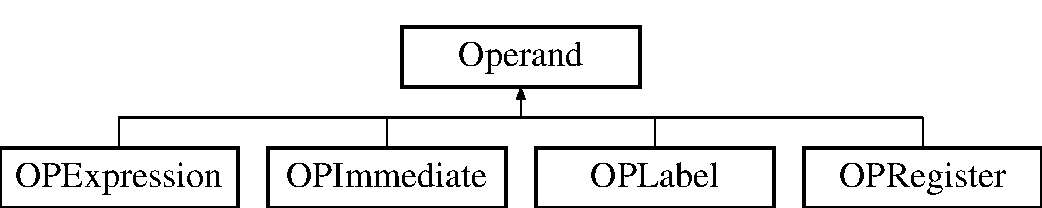
\includegraphics[height=2cm]{classOperand}
\end{center}
\end{figure}
\subsection*{Public Member Functions}
\begin{DoxyCompactItemize}
\item 
\hypertarget{classOperand_aa6ef1ffa183381edb413f9b93782a67b}{
virtual \hyperlink{classOperand_aa6ef1ffa183381edb413f9b93782a67b}{$\sim$Operand} ()}
\label{classOperand_aa6ef1ffa183381edb413f9b93782a67b}

\begin{DoxyCompactList}\small\item\em Virtual destructor. \item\end{DoxyCompactList}\item 
\hypertarget{classOperand_a8cf27955648cbf07144abf4e5a77c266}{
virtual string \hyperlink{classOperand_a8cf27955648cbf07144abf4e5a77c266}{getOp} ()=0}
\label{classOperand_a8cf27955648cbf07144abf4e5a77c266}

\begin{DoxyCompactList}\small\item\em Get the operand value virtual accessor of the operand. \item\end{DoxyCompactList}\item 
\hypertarget{classOperand_a9c31a741d9c16506a9e6c9217e205bd0}{
virtual void \hyperlink{classOperand_a9c31a741d9c16506a9e6c9217e205bd0}{setOp} (string)=0}
\label{classOperand_a9c31a741d9c16506a9e6c9217e205bd0}

\begin{DoxyCompactList}\small\item\em set the operand value virtual setter of the operand \item\end{DoxyCompactList}\item 
virtual t\_\-OpType \hyperlink{classOperand_af4bd7dab87bfd7f3c17ea84f07b02b69}{getOptype} ()=0
\begin{DoxyCompactList}\small\item\em get the operator type virtual accessor of accessor \item\end{DoxyCompactList}\item 
virtual string \hyperlink{classOperand_aaa9879d6c4fb8334c1b4d97dad614cef}{toString} ()=0
\begin{DoxyCompactList}\small\item\em virtual tostring \item\end{DoxyCompactList}\item 
\hypertarget{classOperand_af9f77597fd0bfb387989fae7acf71957}{
virtual t\_\-Src\_\-Dst \hyperlink{classOperand_af9f77597fd0bfb387989fae7acf71957}{getType} ()=0}
\label{classOperand_af9f77597fd0bfb387989fae7acf71957}

\begin{DoxyCompactList}\small\item\em get the type of the register getter of the register type \item\end{DoxyCompactList}\end{DoxyCompactItemize}
\subsection*{Protected Attributes}
\begin{DoxyCompactItemize}
\item 
\hypertarget{classOperand_af70a183445064a0106d41dfeea681790}{
string {\bfseries \_\-oper}}
\label{classOperand_af70a183445064a0106d41dfeea681790}

\end{DoxyCompactItemize}


\subsection{Detailed Description}
Abstract class representing an operand. 

\subsection{Member Function Documentation}
\hypertarget{classOperand_af4bd7dab87bfd7f3c17ea84f07b02b69}{
\index{Operand@{Operand}!getOptype@{getOptype}}
\index{getOptype@{getOptype}!Operand@{Operand}}
\subsubsection[{getOptype}]{\setlength{\rightskip}{0pt plus 5cm}virtual t\_\-OpType Operand::getOptype ()\hspace{0.3cm}{\ttfamily  \mbox{[}pure virtual\mbox{]}}}}
\label{classOperand_af4bd7dab87bfd7f3c17ea84f07b02b69}


get the operator type virtual accessor of accessor \begin{DoxyReturn}{Returns}
return the \hyperlink{classOperand}{Operand} type as enum 
\end{DoxyReturn}


Implemented in \hyperlink{classOPExpression_a26efe8d14f0d37157c885ff16988be30}{OPExpression}, \hyperlink{classOPImmediate_af637aedc23b19948b3b2a3de80b730e7}{OPImmediate}, \hyperlink{classOPLabel_a840489088fc49c57b02264089ec4c55b}{OPLabel}, and \hyperlink{classOPRegister_a06690941f531390e7d71526244c0812b}{OPRegister}.\hypertarget{classOperand_aaa9879d6c4fb8334c1b4d97dad614cef}{
\index{Operand@{Operand}!toString@{toString}}
\index{toString@{toString}!Operand@{Operand}}
\subsubsection[{toString}]{\setlength{\rightskip}{0pt plus 5cm}virtual string Operand::toString ()\hspace{0.3cm}{\ttfamily  \mbox{[}pure virtual\mbox{]}}}}
\label{classOperand_aaa9879d6c4fb8334c1b4d97dad614cef}


virtual tostring \begin{DoxyReturn}{Returns}
return the Object as string 
\end{DoxyReturn}


Implemented in \hyperlink{classOPExpression_a6a29cfb44936766a61099835482ea6d1}{OPExpression}, \hyperlink{classOPImmediate_adbf4bcd0bd6be9d6cb0dcbc5e09ff900}{OPImmediate}, \hyperlink{classOPLabel_a94c9cdc5cf0b3af05a1f917c0d650056}{OPLabel}, and \hyperlink{classOPRegister_a233e4744403c78afc8e88e4c804a485f}{OPRegister}.

The documentation for this class was generated from the following file:\begin{DoxyCompactItemize}
\item 
\hyperlink{Operand_8h}{Operand.h}\end{DoxyCompactItemize}

\hypertarget{classOPExpression}{
\section{OPExpression Class Reference}
\label{classOPExpression}\index{OPExpression@{OPExpression}}
}


class representing an expression herited by \hyperlink{classOperand}{Operand}  


{\ttfamily \#include $<$OPExpression.h$>$}Inheritance diagram for OPExpression::\begin{figure}[H]
\begin{center}
\leavevmode
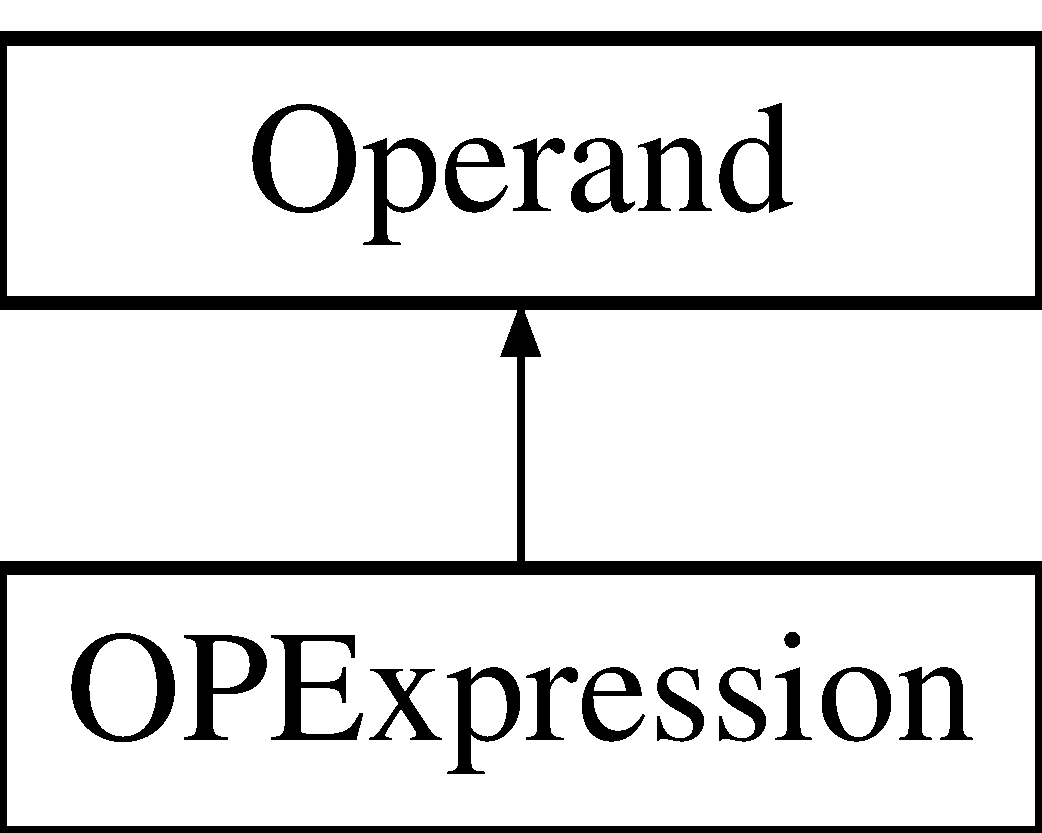
\includegraphics[height=2cm]{classOPExpression}
\end{center}
\end{figure}
\subsection*{Public Member Functions}
\begin{DoxyCompactItemize}
\item 
\hypertarget{classOPExpression_a5784034daef8568869fe0bb5ecfbcdcf}{
\hyperlink{classOPExpression_a5784034daef8568869fe0bb5ecfbcdcf}{OPExpression} (string)}
\label{classOPExpression_a5784034daef8568869fe0bb5ecfbcdcf}

\begin{DoxyCompactList}\small\item\em Constructor of the Expression class. \item\end{DoxyCompactList}\item 
\hypertarget{classOPExpression_a5ea892d89208ccb593510ee63ef42a19}{
virtual \hyperlink{classOPExpression_a5ea892d89208ccb593510ee63ef42a19}{$\sim$OPExpression} ()}
\label{classOPExpression_a5ea892d89208ccb593510ee63ef42a19}

\begin{DoxyCompactList}\small\item\em Destructor of the Expression class. \item\end{DoxyCompactList}\item 
virtual string \hyperlink{classOPExpression_a7b095019f9c2138f1f6bfd21bf4348d9}{getOp} ()
\begin{DoxyCompactList}\small\item\em Get the operand value. \item\end{DoxyCompactList}\item 
virtual t\_\-OpType \hyperlink{classOPExpression_a26efe8d14f0d37157c885ff16988be30}{getOptype} ()
\begin{DoxyCompactList}\small\item\em get the operator type \item\end{DoxyCompactList}\item 
virtual string \hyperlink{classOPExpression_a6a29cfb44936766a61099835482ea6d1}{toString} ()
\begin{DoxyCompactList}\small\item\em tostring \item\end{DoxyCompactList}\item 
\hypertarget{classOPExpression_a5bfc431b31030e3439bda2c7648374b0}{
virtual void \hyperlink{classOPExpression_a5bfc431b31030e3439bda2c7648374b0}{setOp} (string)}
\label{classOPExpression_a5bfc431b31030e3439bda2c7648374b0}

\begin{DoxyCompactList}\small\item\em set the operand value setter of the operand \item\end{DoxyCompactList}\item 
\hypertarget{classOPExpression_accdf986185c7d8261a53bd4ec00370fc}{
virtual t\_\-Src\_\-Dst \hyperlink{classOPExpression_accdf986185c7d8261a53bd4ec00370fc}{getType} ()}
\label{classOPExpression_accdf986185c7d8261a53bd4ec00370fc}

\begin{DoxyCompactList}\small\item\em get the Dst/Src type of the \hyperlink{classOperand}{Operand} getter of the type \item\end{DoxyCompactList}\end{DoxyCompactItemize}


\subsection{Detailed Description}
class representing an expression herited by \hyperlink{classOperand}{Operand} 

\subsection{Member Function Documentation}
\hypertarget{classOPExpression_a7b095019f9c2138f1f6bfd21bf4348d9}{
\index{OPExpression@{OPExpression}!getOp@{getOp}}
\index{getOp@{getOp}!OPExpression@{OPExpression}}
\subsubsection[{getOp}]{\setlength{\rightskip}{0pt plus 5cm}virtual string OPExpression::getOp ()\hspace{0.3cm}{\ttfamily  \mbox{[}virtual\mbox{]}}}}
\label{classOPExpression_a7b095019f9c2138f1f6bfd21bf4348d9}


Get the operand value. \begin{DoxyReturn}{Returns}
return the string of the Expression 
\end{DoxyReturn}


Implements \hyperlink{classOperand_a8cf27955648cbf07144abf4e5a77c266}{Operand}.\hypertarget{classOPExpression_a26efe8d14f0d37157c885ff16988be30}{
\index{OPExpression@{OPExpression}!getOptype@{getOptype}}
\index{getOptype@{getOptype}!OPExpression@{OPExpression}}
\subsubsection[{getOptype}]{\setlength{\rightskip}{0pt plus 5cm}virtual t\_\-OpType OPExpression::getOptype ()\hspace{0.3cm}{\ttfamily  \mbox{[}virtual\mbox{]}}}}
\label{classOPExpression_a26efe8d14f0d37157c885ff16988be30}


get the operator type \begin{DoxyReturn}{Returns}
return the \hyperlink{classOperand}{Operand} type as enum 
\end{DoxyReturn}


Implements \hyperlink{classOperand_af4bd7dab87bfd7f3c17ea84f07b02b69}{Operand}.\hypertarget{classOPExpression_a6a29cfb44936766a61099835482ea6d1}{
\index{OPExpression@{OPExpression}!toString@{toString}}
\index{toString@{toString}!OPExpression@{OPExpression}}
\subsubsection[{toString}]{\setlength{\rightskip}{0pt plus 5cm}virtual string OPExpression::toString ()\hspace{0.3cm}{\ttfamily  \mbox{[}virtual\mbox{]}}}}
\label{classOPExpression_a6a29cfb44936766a61099835482ea6d1}


tostring \begin{DoxyReturn}{Returns}
return the Object as string 
\end{DoxyReturn}


Implements \hyperlink{classOperand_aaa9879d6c4fb8334c1b4d97dad614cef}{Operand}.

The documentation for this class was generated from the following file:\begin{DoxyCompactItemize}
\item 
\hyperlink{OPExpression_8h}{OPExpression.h}\end{DoxyCompactItemize}

\hypertarget{classOPImmediate}{
\section{OPImmediate Class Reference}
\label{classOPImmediate}\index{OPImmediate@{OPImmediate}}
}


class representing an Immediate herited by \hyperlink{classOperand}{Operand}  


{\ttfamily \#include $<$OPImmediate.h$>$}Inheritance diagram for OPImmediate::\begin{figure}[H]
\begin{center}
\leavevmode
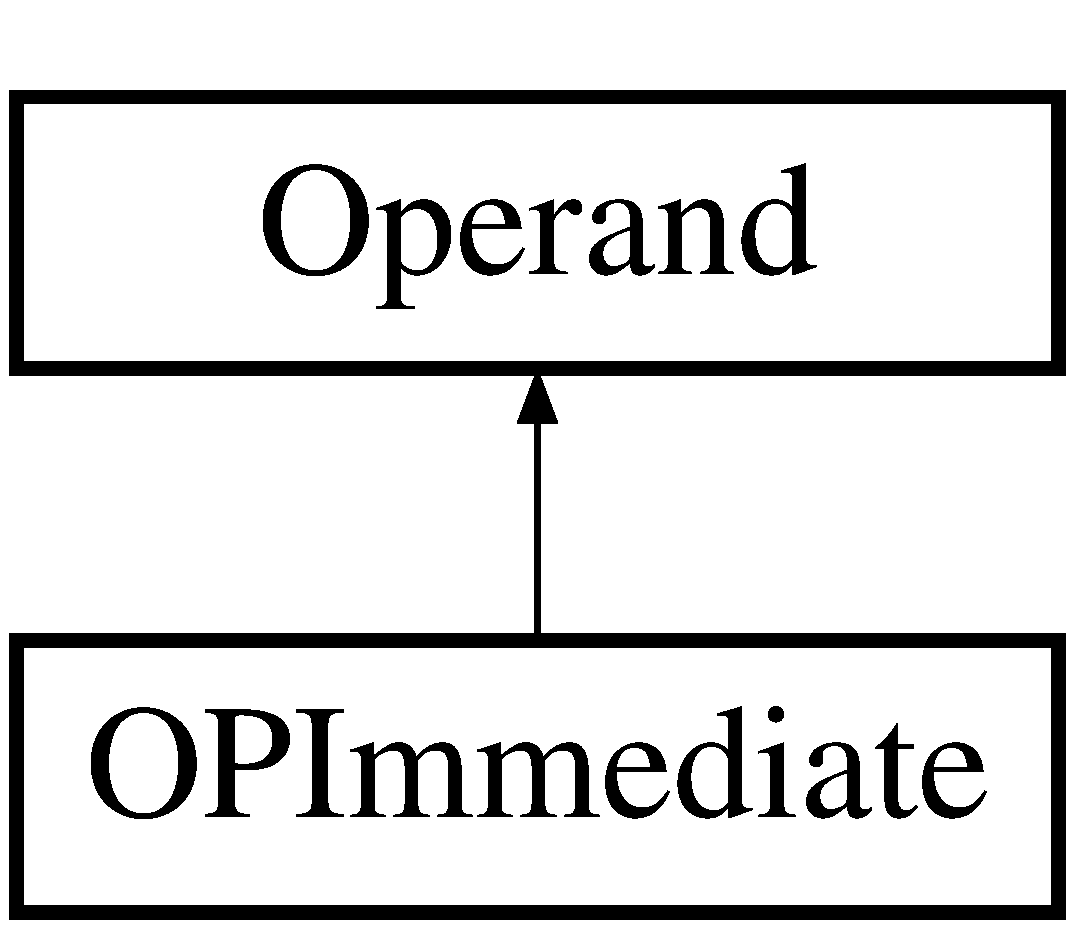
\includegraphics[height=2cm]{classOPImmediate}
\end{center}
\end{figure}
\subsection*{Public Member Functions}
\begin{DoxyCompactItemize}
\item 
\hypertarget{classOPImmediate_ab047dac5f3390947a21e4ab118c05857}{
\hyperlink{classOPImmediate_ab047dac5f3390947a21e4ab118c05857}{OPImmediate} (string)}
\label{classOPImmediate_ab047dac5f3390947a21e4ab118c05857}

\begin{DoxyCompactList}\small\item\em Constructor of the Immediate Class. \item\end{DoxyCompactList}\item 
\hypertarget{classOPImmediate_ae940dcf9e9050227a94c759a0cae6861}{
\hyperlink{classOPImmediate_ae940dcf9e9050227a94c759a0cae6861}{OPImmediate} (int)}
\label{classOPImmediate_ae940dcf9e9050227a94c759a0cae6861}

\begin{DoxyCompactList}\small\item\em Constructor of the Immediate Class. \item\end{DoxyCompactList}\item 
\hypertarget{classOPImmediate_af7f51ae61e075e02817d6ecd7441408f}{
virtual \hyperlink{classOPImmediate_af7f51ae61e075e02817d6ecd7441408f}{$\sim$OPImmediate} ()}
\label{classOPImmediate_af7f51ae61e075e02817d6ecd7441408f}

\begin{DoxyCompactList}\small\item\em Destructor of the Immediate Class. \item\end{DoxyCompactList}\item 
virtual string \hyperlink{classOPImmediate_a36a14a13ac2dde34bba3d31cfd474f9b}{getOp} ()
\begin{DoxyCompactList}\small\item\em Get the string of the operand. \item\end{DoxyCompactList}\item 
virtual t\_\-OpType \hyperlink{classOPImmediate_af637aedc23b19948b3b2a3de80b730e7}{getOptype} ()
\begin{DoxyCompactList}\small\item\em get the operator type \item\end{DoxyCompactList}\item 
virtual string \hyperlink{classOPImmediate_adbf4bcd0bd6be9d6cb0dcbc5e09ff900}{toString} ()
\begin{DoxyCompactList}\small\item\em tostring \item\end{DoxyCompactList}\item 
\hypertarget{classOPImmediate_a3fe67ad761df93fb741c3837f1cc5711}{
virtual void \hyperlink{classOPImmediate_a3fe67ad761df93fb741c3837f1cc5711}{setOp} (string)}
\label{classOPImmediate_a3fe67ad761df93fb741c3837f1cc5711}

\begin{DoxyCompactList}\small\item\em set the string of the operand setter of the operand \item\end{DoxyCompactList}\item 
\hypertarget{classOPImmediate_a21f9307817b2a14e642f94e5175b925a}{
virtual t\_\-Src\_\-Dst \hyperlink{classOPImmediate_a21f9307817b2a14e642f94e5175b925a}{getType} ()}
\label{classOPImmediate_a21f9307817b2a14e642f94e5175b925a}

\begin{DoxyCompactList}\small\item\em get the Dst/Src type of the \hyperlink{classOperand}{Operand} getter of the type \item\end{DoxyCompactList}\end{DoxyCompactItemize}


\subsection{Detailed Description}
class representing an Immediate herited by \hyperlink{classOperand}{Operand} 

\subsection{Member Function Documentation}
\hypertarget{classOPImmediate_a36a14a13ac2dde34bba3d31cfd474f9b}{
\index{OPImmediate@{OPImmediate}!getOp@{getOp}}
\index{getOp@{getOp}!OPImmediate@{OPImmediate}}
\subsubsection[{getOp}]{\setlength{\rightskip}{0pt plus 5cm}virtual string OPImmediate::getOp ()\hspace{0.3cm}{\ttfamily  \mbox{[}virtual\mbox{]}}}}
\label{classOPImmediate_a36a14a13ac2dde34bba3d31cfd474f9b}


Get the string of the operand. \begin{DoxyReturn}{Returns}
return the string of the Immediate 
\end{DoxyReturn}


Implements \hyperlink{classOperand_a8cf27955648cbf07144abf4e5a77c266}{Operand}.\hypertarget{classOPImmediate_af637aedc23b19948b3b2a3de80b730e7}{
\index{OPImmediate@{OPImmediate}!getOptype@{getOptype}}
\index{getOptype@{getOptype}!OPImmediate@{OPImmediate}}
\subsubsection[{getOptype}]{\setlength{\rightskip}{0pt plus 5cm}virtual t\_\-OpType OPImmediate::getOptype ()\hspace{0.3cm}{\ttfamily  \mbox{[}virtual\mbox{]}}}}
\label{classOPImmediate_af637aedc23b19948b3b2a3de80b730e7}


get the operator type \begin{DoxyReturn}{Returns}
return the \hyperlink{classOperand}{Operand} type as enum 
\end{DoxyReturn}


Implements \hyperlink{classOperand_af4bd7dab87bfd7f3c17ea84f07b02b69}{Operand}.\hypertarget{classOPImmediate_adbf4bcd0bd6be9d6cb0dcbc5e09ff900}{
\index{OPImmediate@{OPImmediate}!toString@{toString}}
\index{toString@{toString}!OPImmediate@{OPImmediate}}
\subsubsection[{toString}]{\setlength{\rightskip}{0pt plus 5cm}virtual string OPImmediate::toString ()\hspace{0.3cm}{\ttfamily  \mbox{[}virtual\mbox{]}}}}
\label{classOPImmediate_adbf4bcd0bd6be9d6cb0dcbc5e09ff900}


tostring \begin{DoxyReturn}{Returns}
return the name of the Object as string 
\end{DoxyReturn}


Implements \hyperlink{classOperand_aaa9879d6c4fb8334c1b4d97dad614cef}{Operand}.

The documentation for this class was generated from the following file:\begin{DoxyCompactItemize}
\item 
\hyperlink{OPImmediate_8h}{OPImmediate.h}\end{DoxyCompactItemize}

\hypertarget{classOPLabel}{
\section{OPLabel Class Reference}
\label{classOPLabel}\index{OPLabel@{OPLabel}}
}


class representing a \hyperlink{classLabel}{Label} herited by \hyperlink{classOperand}{Operand}  


{\ttfamily \#include $<$OPLabel.h$>$}Inheritance diagram for OPLabel::\begin{figure}[H]
\begin{center}
\leavevmode
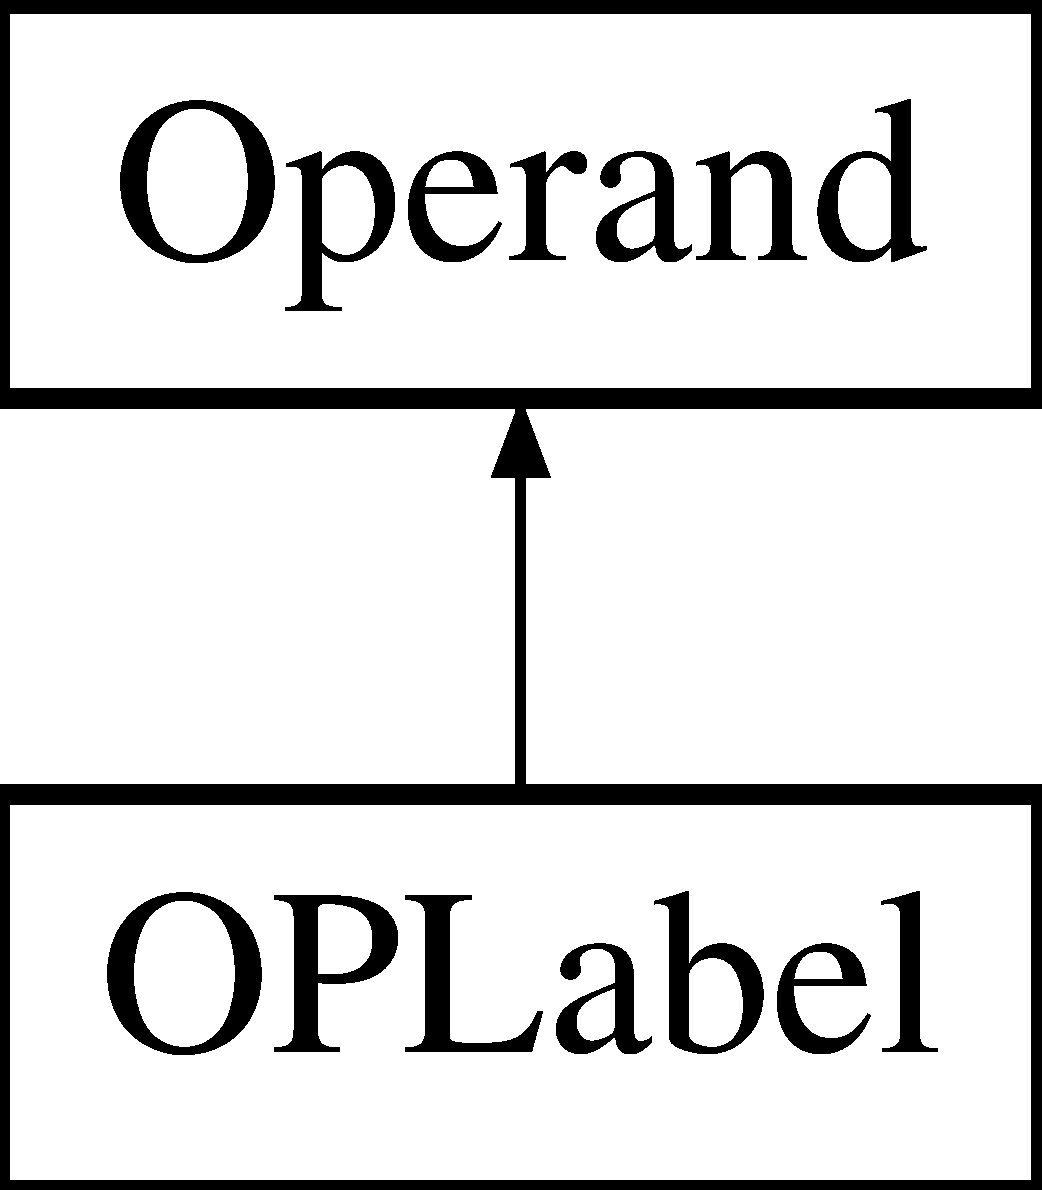
\includegraphics[height=2cm]{classOPLabel}
\end{center}
\end{figure}
\subsection*{Public Member Functions}
\begin{DoxyCompactItemize}
\item 
\hypertarget{classOPLabel_a5405b78894658047362a328e750f88b4}{
\hyperlink{classOPLabel_a5405b78894658047362a328e750f88b4}{OPLabel} (string)}
\label{classOPLabel_a5405b78894658047362a328e750f88b4}

\begin{DoxyCompactList}\small\item\em Constructor of the \hyperlink{classLabel}{Label} Class. \item\end{DoxyCompactList}\item 
\hypertarget{classOPLabel_ab25553d41606e880a622e09d5c09129d}{
virtual \hyperlink{classOPLabel_ab25553d41606e880a622e09d5c09129d}{$\sim$OPLabel} ()}
\label{classOPLabel_ab25553d41606e880a622e09d5c09129d}

\begin{DoxyCompactList}\small\item\em Destructor of the \hyperlink{classLabel}{Label} Class. \item\end{DoxyCompactList}\item 
\hypertarget{classOPLabel_aa41863a748c2fad74e219da9681932e7}{
virtual string \hyperlink{classOPLabel_aa41863a748c2fad74e219da9681932e7}{getOp} ()}
\label{classOPLabel_aa41863a748c2fad74e219da9681932e7}

\begin{DoxyCompactList}\small\item\em Get the string of the operand accessor of the operand. \item\end{DoxyCompactList}\item 
virtual t\_\-OpType \hyperlink{classOPLabel_a840489088fc49c57b02264089ec4c55b}{getOptype} ()
\begin{DoxyCompactList}\small\item\em get the operator type \item\end{DoxyCompactList}\item 
virtual string \hyperlink{classOPLabel_a94c9cdc5cf0b3af05a1f917c0d650056}{toString} ()
\begin{DoxyCompactList}\small\item\em tostring \item\end{DoxyCompactList}\item 
\hypertarget{classOPLabel_a10e5dfb1f7b2eee9f2327cd2601ed9be}{
virtual void \hyperlink{classOPLabel_a10e5dfb1f7b2eee9f2327cd2601ed9be}{setOp} (string)}
\label{classOPLabel_a10e5dfb1f7b2eee9f2327cd2601ed9be}

\begin{DoxyCompactList}\small\item\em set the operand value setter of the operand \item\end{DoxyCompactList}\item 
\hypertarget{classOPLabel_a602f62f783c370402b4841b0aed1f307}{
virtual t\_\-Src\_\-Dst \hyperlink{classOPLabel_a602f62f783c370402b4841b0aed1f307}{getType} ()}
\label{classOPLabel_a602f62f783c370402b4841b0aed1f307}

\begin{DoxyCompactList}\small\item\em get the Dst/Src type of the \hyperlink{classOperand}{Operand} getter of the type \item\end{DoxyCompactList}\end{DoxyCompactItemize}


\subsection{Detailed Description}
class representing a \hyperlink{classLabel}{Label} herited by \hyperlink{classOperand}{Operand} 

\subsection{Member Function Documentation}
\hypertarget{classOPLabel_a840489088fc49c57b02264089ec4c55b}{
\index{OPLabel@{OPLabel}!getOptype@{getOptype}}
\index{getOptype@{getOptype}!OPLabel@{OPLabel}}
\subsubsection[{getOptype}]{\setlength{\rightskip}{0pt plus 5cm}virtual t\_\-OpType OPLabel::getOptype ()\hspace{0.3cm}{\ttfamily  \mbox{[}virtual\mbox{]}}}}
\label{classOPLabel_a840489088fc49c57b02264089ec4c55b}


get the operator type \begin{DoxyReturn}{Returns}
return the \hyperlink{classOperand}{Operand} type as enum 
\end{DoxyReturn}


Implements \hyperlink{classOperand_af4bd7dab87bfd7f3c17ea84f07b02b69}{Operand}.\hypertarget{classOPLabel_a94c9cdc5cf0b3af05a1f917c0d650056}{
\index{OPLabel@{OPLabel}!toString@{toString}}
\index{toString@{toString}!OPLabel@{OPLabel}}
\subsubsection[{toString}]{\setlength{\rightskip}{0pt plus 5cm}virtual string OPLabel::toString ()\hspace{0.3cm}{\ttfamily  \mbox{[}virtual\mbox{]}}}}
\label{classOPLabel_a94c9cdc5cf0b3af05a1f917c0d650056}


tostring \begin{DoxyReturn}{Returns}
return the name of the Object as string 
\end{DoxyReturn}


Implements \hyperlink{classOperand_aaa9879d6c4fb8334c1b4d97dad614cef}{Operand}.

The documentation for this class was generated from the following file:\begin{DoxyCompactItemize}
\item 
\hyperlink{OPLabel_8h}{OPLabel.h}\end{DoxyCompactItemize}

\hypertarget{classOPRegister}{
\section{OPRegister Class Reference}
\label{classOPRegister}\index{OPRegister@{OPRegister}}
}


class representing a Register herited by \hyperlink{classOperand}{Operand}  


{\ttfamily \#include $<$OPRegister.h$>$}Inheritance diagram for OPRegister::\begin{figure}[H]
\begin{center}
\leavevmode
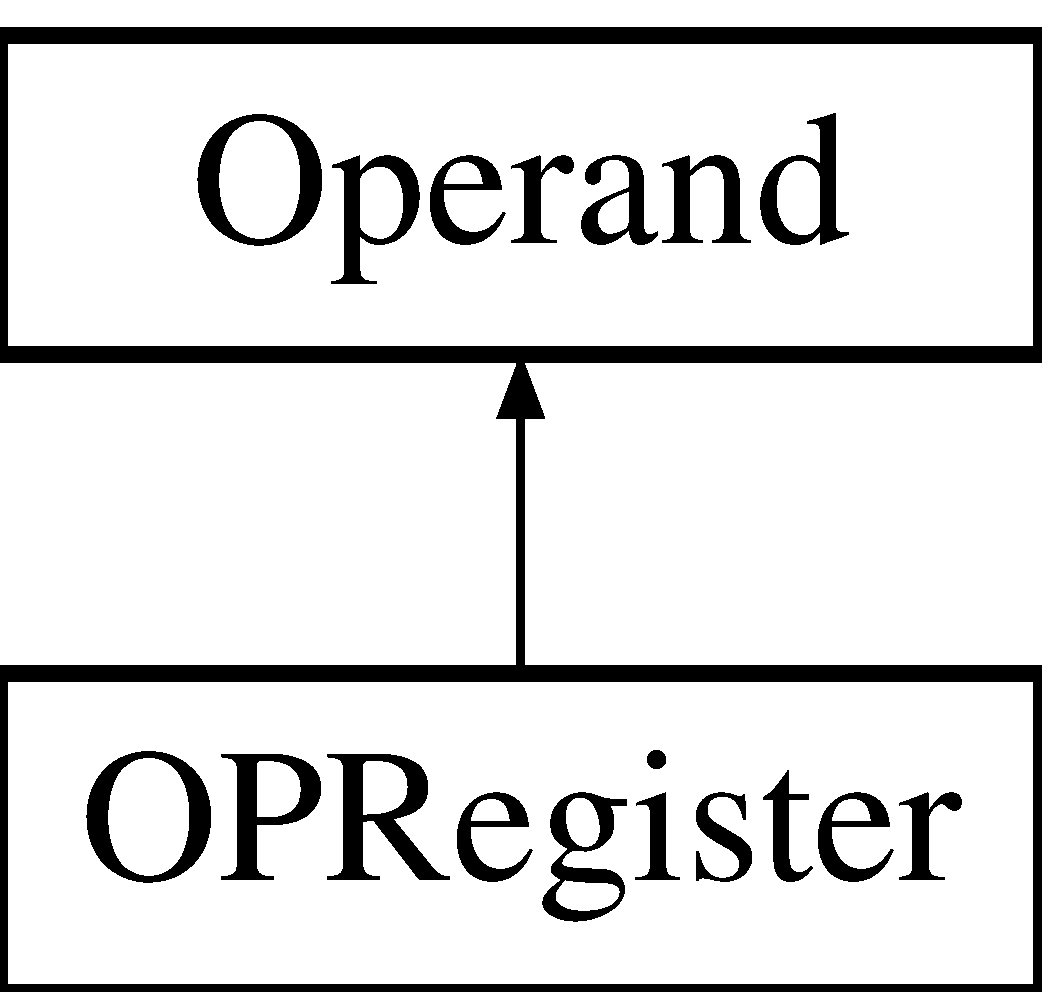
\includegraphics[height=2cm]{classOPRegister}
\end{center}
\end{figure}
\subsection*{Public Member Functions}
\begin{DoxyCompactItemize}
\item 
\hypertarget{classOPRegister_a896eb65f36bf615ccfa74541de23858f}{
\hyperlink{classOPRegister_a896eb65f36bf615ccfa74541de23858f}{OPRegister} (string, t\_\-Src\_\-Dst)}
\label{classOPRegister_a896eb65f36bf615ccfa74541de23858f}

\begin{DoxyCompactList}\small\item\em Constructor of the Register class. \item\end{DoxyCompactList}\item 
\hypertarget{classOPRegister_ad75c23d1db7c149c20cbc8bb01c6df59}{
\hyperlink{classOPRegister_ad75c23d1db7c149c20cbc8bb01c6df59}{OPRegister} (string, int, t\_\-Src\_\-Dst)}
\label{classOPRegister_ad75c23d1db7c149c20cbc8bb01c6df59}

\begin{DoxyCompactList}\small\item\em Constructor of the Register class. \item\end{DoxyCompactList}\item 
\hypertarget{classOPRegister_a3c9786680764ada47370d469790b8178}{
{\bfseries OPRegister} (int, t\_\-Src\_\-Dst)}
\label{classOPRegister_a3c9786680764ada47370d469790b8178}

\item 
\hypertarget{classOPRegister_aedab3bc5a2eecd0d02771fb6b37d73fe}{
virtual \hyperlink{classOPRegister_aedab3bc5a2eecd0d02771fb6b37d73fe}{$\sim$OPRegister} ()}
\label{classOPRegister_aedab3bc5a2eecd0d02771fb6b37d73fe}

\begin{DoxyCompactList}\small\item\em Destructor of the Register class. \item\end{DoxyCompactList}\item 
int \hyperlink{classOPRegister_af409289a33aff7c3d0469d748aeacd15}{getReg} ()
\begin{DoxyCompactList}\small\item\em Get the Register value. \item\end{DoxyCompactList}\item 
\hypertarget{classOPRegister_a2e9b7e1d1b23360357573c95dc89e35b}{
void \hyperlink{classOPRegister_a2e9b7e1d1b23360357573c95dc89e35b}{setReg} (int)}
\label{classOPRegister_a2e9b7e1d1b23360357573c95dc89e35b}

\begin{DoxyCompactList}\small\item\em set the Register value setter of the Register \item\end{DoxyCompactList}\item 
virtual string \hyperlink{classOPRegister_a660f194996324eb71a3db0cbdccdab49}{getOp} ()
\begin{DoxyCompactList}\small\item\em Get the operand value. \item\end{DoxyCompactList}\item 
virtual t\_\-OpType \hyperlink{classOPRegister_a06690941f531390e7d71526244c0812b}{getOptype} ()
\begin{DoxyCompactList}\small\item\em get the operator type \item\end{DoxyCompactList}\item 
virtual string \hyperlink{classOPRegister_a233e4744403c78afc8e88e4c804a485f}{toString} ()
\begin{DoxyCompactList}\small\item\em tostring \item\end{DoxyCompactList}\item 
\hypertarget{classOPRegister_a7ef4a1673a14a98f6fbe30585781bdec}{
virtual void \hyperlink{classOPRegister_a7ef4a1673a14a98f6fbe30585781bdec}{setOp} (string)}
\label{classOPRegister_a7ef4a1673a14a98f6fbe30585781bdec}

\begin{DoxyCompactList}\small\item\em set the operand value setter of the operand \item\end{DoxyCompactList}\item 
\hypertarget{classOPRegister_aed2369f4a27d3033548a7be15ed34cfa}{
void \hyperlink{classOPRegister_aed2369f4a27d3033548a7be15ed34cfa}{setType} (t\_\-Src\_\-Dst)}
\label{classOPRegister_aed2369f4a27d3033548a7be15ed34cfa}

\begin{DoxyCompactList}\small\item\em set the type of the register setter of the register type \item\end{DoxyCompactList}\item 
\hypertarget{classOPRegister_a4b8d1403aab343f1fd599b5bfa437f76}{
virtual t\_\-Src\_\-Dst \hyperlink{classOPRegister_a4b8d1403aab343f1fd599b5bfa437f76}{getType} ()}
\label{classOPRegister_a4b8d1403aab343f1fd599b5bfa437f76}

\begin{DoxyCompactList}\small\item\em get the type of the register getter of the register type \item\end{DoxyCompactList}\end{DoxyCompactItemize}


\subsection{Detailed Description}
class representing a Register herited by \hyperlink{classOperand}{Operand} 

\subsection{Member Function Documentation}
\hypertarget{classOPRegister_a660f194996324eb71a3db0cbdccdab49}{
\index{OPRegister@{OPRegister}!getOp@{getOp}}
\index{getOp@{getOp}!OPRegister@{OPRegister}}
\subsubsection[{getOp}]{\setlength{\rightskip}{0pt plus 5cm}virtual string OPRegister::getOp ()\hspace{0.3cm}{\ttfamily  \mbox{[}virtual\mbox{]}}}}
\label{classOPRegister_a660f194996324eb71a3db0cbdccdab49}


Get the operand value. \begin{DoxyReturn}{Returns}
return the string of the register 
\end{DoxyReturn}


Implements \hyperlink{classOperand_a8cf27955648cbf07144abf4e5a77c266}{Operand}.\hypertarget{classOPRegister_a06690941f531390e7d71526244c0812b}{
\index{OPRegister@{OPRegister}!getOptype@{getOptype}}
\index{getOptype@{getOptype}!OPRegister@{OPRegister}}
\subsubsection[{getOptype}]{\setlength{\rightskip}{0pt plus 5cm}virtual t\_\-OpType OPRegister::getOptype ()\hspace{0.3cm}{\ttfamily  \mbox{[}virtual\mbox{]}}}}
\label{classOPRegister_a06690941f531390e7d71526244c0812b}


get the operator type \begin{DoxyReturn}{Returns}
return the \hyperlink{classOperand}{Operand} type as enum 
\end{DoxyReturn}


Implements \hyperlink{classOperand_af4bd7dab87bfd7f3c17ea84f07b02b69}{Operand}.\hypertarget{classOPRegister_af409289a33aff7c3d0469d748aeacd15}{
\index{OPRegister@{OPRegister}!getReg@{getReg}}
\index{getReg@{getReg}!OPRegister@{OPRegister}}
\subsubsection[{getReg}]{\setlength{\rightskip}{0pt plus 5cm}int OPRegister::getReg ()}}
\label{classOPRegister_af409289a33aff7c3d0469d748aeacd15}


Get the Register value. \begin{DoxyReturn}{Returns}
return the number of the Register 
\end{DoxyReturn}
\hypertarget{classOPRegister_a233e4744403c78afc8e88e4c804a485f}{
\index{OPRegister@{OPRegister}!toString@{toString}}
\index{toString@{toString}!OPRegister@{OPRegister}}
\subsubsection[{toString}]{\setlength{\rightskip}{0pt plus 5cm}virtual string OPRegister::toString ()\hspace{0.3cm}{\ttfamily  \mbox{[}virtual\mbox{]}}}}
\label{classOPRegister_a233e4744403c78afc8e88e4c804a485f}


tostring \begin{DoxyReturn}{Returns}
return the Object as string 
\end{DoxyReturn}


Implements \hyperlink{classOperand_aaa9879d6c4fb8334c1b4d97dad614cef}{Operand}.

The documentation for this class was generated from the following file:\begin{DoxyCompactItemize}
\item 
\hyperlink{OPRegister_8h}{OPRegister.h}\end{DoxyCompactItemize}

\hypertarget{classProgram}{
\section{Program Class Reference}
\label{classProgram}\index{Program@{Program}}
}


class representing a program as list  


{\ttfamily \#include $<$Program.h$>$}\subsection*{Public Member Functions}
\begin{DoxyCompactItemize}
\item 
\hypertarget{classProgram_aaefaa0df08f3484476fc4d61e97acbdc}{
\hyperlink{classProgram_aaefaa0df08f3484476fc4d61e97acbdc}{Program} ()}
\label{classProgram_aaefaa0df08f3484476fc4d61e97acbdc}

\begin{DoxyCompactList}\small\item\em Empty constructor of program. \item\end{DoxyCompactList}\item 
\hypertarget{classProgram_a9918fe797bf830c47a652c81f449c35c}{
\hyperlink{classProgram_a9918fe797bf830c47a652c81f449c35c}{Program} (\hyperlink{classProgram}{Program} const \&otherprogram)}
\label{classProgram_a9918fe797bf830c47a652c81f449c35c}

\begin{DoxyCompactList}\small\item\em Copy constructor of program. \item\end{DoxyCompactList}\item 
\hypertarget{classProgram_a8db47dbd7d0c03848cd4cb75be785088}{
\hyperlink{classProgram_a8db47dbd7d0c03848cd4cb75be785088}{Program} (FILE $\ast$sourceasm)}
\label{classProgram_a8db47dbd7d0c03848cd4cb75be785088}

\begin{DoxyCompactList}\small\item\em Constructor with input file of program. \item\end{DoxyCompactList}\item 
\hypertarget{classProgram_a986aef1c50e1d338a3315a47ba6df549}{
\hyperlink{classProgram_a986aef1c50e1d338a3315a47ba6df549}{$\sim$Program} ()}
\label{classProgram_a986aef1c50e1d338a3315a47ba6df549}

\begin{DoxyCompactList}\small\item\em Destructor of program. \item\end{DoxyCompactList}\item 
\hypertarget{classProgram_a3f0df57e5b726978cc2194c94cc76d18}{
void \hyperlink{classProgram_a3f0df57e5b726978cc2194c94cc76d18}{addLine} (\hyperlink{classLine}{Line} $\ast$newline)}
\label{classProgram_a3f0df57e5b726978cc2194c94cc76d18}

\begin{DoxyCompactList}\small\item\em Add a line at the end of the program. \item\end{DoxyCompactList}\item 
\hypertarget{classProgram_aea3d46bd7c1908ce9b253f0140345eaa}{
int \hyperlink{classProgram_aea3d46bd7c1908ce9b253f0140345eaa}{add\_\-Line\_\-at} (\hyperlink{classLine}{Line} $\ast$newline, int position)}
\label{classProgram_aea3d46bd7c1908ce9b253f0140345eaa}

\begin{DoxyCompactList}\small\item\em Add a line to the program with position as index. \item\end{DoxyCompactList}\item 
\hypertarget{classProgram_a3c1399ac5ed69e5c152f1a2cc1e644d4}{
void \hyperlink{classProgram_a3c1399ac5ed69e5c152f1a2cc1e644d4}{display} ()}
\label{classProgram_a3c1399ac5ed69e5c152f1a2cc1e644d4}

\begin{DoxyCompactList}\small\item\em display the program \item\end{DoxyCompactList}\item 
\hypertarget{classProgram_a08dffa0f779f1ce089649c73d5e44498}{
void \hyperlink{classProgram_a08dffa0f779f1ce089649c73d5e44498}{delLine} (int index)}
\label{classProgram_a08dffa0f779f1ce089649c73d5e44498}

\begin{DoxyCompactList}\small\item\em Delete a line in the program. \item\end{DoxyCompactList}\item 
\hypertarget{classProgram_a8f37b171319c0e4a746b4822e4115d23}{
\hyperlink{classLine}{Line} $\ast$ \hyperlink{classProgram_a8f37b171319c0e4a746b4822e4115d23}{findLine} (int index)}
\label{classProgram_a8f37b171319c0e4a746b4822e4115d23}

\begin{DoxyCompactList}\small\item\em gives the line that corresponds to the index \item\end{DoxyCompactList}\item 
\hypertarget{classProgram_a190f24ecadca14d748408c352aabc219}{
int \hyperlink{classProgram_a190f24ecadca14d748408c352aabc219}{size} ()}
\label{classProgram_a190f24ecadca14d748408c352aabc219}

\begin{DoxyCompactList}\small\item\em get the length of the program \item\end{DoxyCompactList}\item 
t\_\-Dep \hyperlink{classProgram_a9626cf3dd2cd7851fb28d84fd6632f52}{dependance} (\hyperlink{classInstruction}{Instruction} i1, \hyperlink{classInstruction}{Instruction} i2)
\begin{DoxyCompactList}\small\item\em get the dependance betwen two instructions \item\end{DoxyCompactList}\item 
\hypertarget{classProgram_a1d7862832ff52e24f864a771b8c2f376}{
void \hyperlink{classProgram_a1d7862832ff52e24f864a771b8c2f376}{inFile} (string const filename)}
\label{classProgram_a1d7862832ff52e24f864a771b8c2f376}

\begin{DoxyCompactList}\small\item\em write the programme in file \item\end{DoxyCompactList}\item 
\hypertarget{classProgram_a4cba05aa33b330dcdaeae7f6d196328a}{
bool \hyperlink{classProgram_a4cba05aa33b330dcdaeae7f6d196328a}{isEmpty} ()}
\label{classProgram_a4cba05aa33b330dcdaeae7f6d196328a}

\begin{DoxyCompactList}\small\item\em return true if the program is Empty \item\end{DoxyCompactList}\item 
\hypertarget{classProgram_a316b99cea93e4ff48c35c72d0ee9f318}{
void \hyperlink{classProgram_a316b99cea93e4ff48c35c72d0ee9f318}{comput\_\-Function} ()}
\label{classProgram_a316b99cea93e4ff48c35c72d0ee9f318}

\begin{DoxyCompactList}\small\item\em calculate functions \item\end{DoxyCompactList}\item 
\hypertarget{classProgram_a49de951941bbf46ca09075109d4d71f0}{
int \hyperlink{classProgram_a49de951941bbf46ca09075109d4d71f0}{nbr\_\-Func} ()}
\label{classProgram_a49de951941bbf46ca09075109d4d71f0}

\begin{DoxyCompactList}\small\item\em get the number of functions in the program \item\end{DoxyCompactList}\item 
\hypertarget{classProgram_a7af654f80023baa51c94604a176355b0}{
\hyperlink{classFunction}{Function} \hyperlink{classProgram_a7af654f80023baa51c94604a176355b0}{get\_\-Function} (int)}
\label{classProgram_a7af654f80023baa51c94604a176355b0}

\begin{DoxyCompactList}\small\item\em get one fonction of the list myfunc \item\end{DoxyCompactList}\end{DoxyCompactItemize}


\subsection{Detailed Description}
class representing a program as list 

\subsection{Member Function Documentation}
\hypertarget{classProgram_a9626cf3dd2cd7851fb28d84fd6632f52}{
\index{Program@{Program}!dependance@{dependance}}
\index{dependance@{dependance}!Program@{Program}}
\subsubsection[{dependance}]{\setlength{\rightskip}{0pt plus 5cm}t\_\-Dep Program::dependance ({\bf Instruction} {\em i1}, \/  {\bf Instruction} {\em i2})}}
\label{classProgram_a9626cf3dd2cd7851fb28d84fd6632f52}


get the dependance betwen two instructions \begin{DoxyReturn}{Returns}
return the dependance in enum format 
\end{DoxyReturn}


The documentation for this class was generated from the following file:\begin{DoxyCompactItemize}
\item 
\hyperlink{Program_8h}{Program.h}\end{DoxyCompactItemize}

\hypertarget{structs__Profile}{
\section{s\_\-Profile Struct Reference}
\label{structs__Profile}\index{s\_\-Profile@{s\_\-Profile}}
}


Structure allowing to add caracteristics to an operator.  


{\ttfamily \#include $<$Enum\_\-type.h$>$}\subsection*{Public Attributes}
\begin{DoxyCompactItemize}
\item 
\hypertarget{structs__Profile_a3debabafa904b8f4c5e7bf2bda2a5e60}{
t\_\-Operator {\bfseries op}}
\label{structs__Profile_a3debabafa904b8f4c5e7bf2bda2a5e60}

\item 
\hypertarget{structs__Profile_ae8153795530389f76f6c56bdeac40d46}{
t\_\-Format {\bfseries format}}
\label{structs__Profile_ae8153795530389f76f6c56bdeac40d46}

\item 
\hypertarget{structs__Profile_a2a8c53bcb4fb28c3aa368a27954d9b1b}{
t\_\-Inst {\bfseries type}}
\label{structs__Profile_a2a8c53bcb4fb28c3aa368a27954d9b1b}

\end{DoxyCompactItemize}


\subsection{Detailed Description}
Structure allowing to add caracteristics to an operator. 

The documentation for this struct was generated from the following file:\begin{DoxyCompactItemize}
\item 
Enum\_\-type.h\end{DoxyCompactItemize}

\hypertarget{classTestOPLabel}{
\section{TestOPLabel Class Reference}
\label{classTestOPLabel}\index{TestOPLabel@{TestOPLabel}}
}
\subsection*{Public Member Functions}
\begin{DoxyCompactItemize}
\item 
\hypertarget{classTestOPLabel_a9ddb0e7ab19700d5bf73490ba0ebbf36}{
void {\bfseries setUp} (void)}
\label{classTestOPLabel_a9ddb0e7ab19700d5bf73490ba0ebbf36}

\item 
\hypertarget{classTestOPLabel_a6bc3fb561309973920fe3abc020facf1}{
void {\bfseries tearDown} (void)}
\label{classTestOPLabel_a6bc3fb561309973920fe3abc020facf1}

\end{DoxyCompactItemize}


The documentation for this class was generated from the following file:\begin{DoxyCompactItemize}
\item 
TestOPLabel.h\end{DoxyCompactItemize}

\hypertarget{structutchn}{
\section{utchn Struct Reference}
\label{structutchn}\index{utchn@{utchn}}
}
\subsection*{Public Attributes}
\begin{DoxyCompactItemize}
\item 
\hypertarget{structutchn_adf89384022b2de9cb3a0be987e746bbe}{
struct \hyperlink{structutchn}{utchn} $\ast$ {\bfseries NEXT}}
\label{structutchn_adf89384022b2de9cb3a0be987e746bbe}

\item 
\hypertarget{structutchn_a4c8453ea9877abcfdb65a88f3497a294}{
union \hyperlink{unionutdat}{utdat} {\bfseries DATA}}
\label{structutchn_a4c8453ea9877abcfdb65a88f3497a294}

\end{DoxyCompactItemize}


The documentation for this struct was generated from the following file:\begin{DoxyCompactItemize}
\item 
utl200.h\end{DoxyCompactItemize}

\hypertarget{unionutdat}{
\section{utdat Union Reference}
\label{unionutdat}\index{utdat@{utdat}}
}
\subsection*{Public Attributes}
\begin{DoxyCompactItemize}
\item 
\hypertarget{unionutdat_a3f76aa32eacd8c9a18af99d01be467c2}{
void $\ast$ {\bfseries VPNT}}
\label{unionutdat_a3f76aa32eacd8c9a18af99d01be467c2}

\item 
\hypertarget{unionutdat_ae0e7486135096802136dc1cd41c9a005}{
float {\bfseries FLOT}}
\label{unionutdat_ae0e7486135096802136dc1cd41c9a005}

\item 
\hypertarget{unionutdat_aae5fc4b76253540a8c4e983e162072be}{
unsigned int {\bfseries UINT}}
\label{unionutdat_aae5fc4b76253540a8c4e983e162072be}

\item 
\hypertarget{unionutdat_a5bf144421cb7bf3264438be37aa5d884}{
int {\bfseries SINT}}
\label{unionutdat_a5bf144421cb7bf3264438be37aa5d884}

\item 
\hypertarget{unionutdat_afad7210b163e44fc45ba5d19f9354b73}{
char {\bfseries CHAR}}
\label{unionutdat_afad7210b163e44fc45ba5d19f9354b73}

\item 
\hypertarget{unionutdat_ac716e252c27e7f050371d9c28b4c75f4}{
unsigned char {\bfseries UCHR}}
\label{unionutdat_ac716e252c27e7f050371d9c28b4c75f4}

\end{DoxyCompactItemize}


The documentation for this union was generated from the following file:\begin{DoxyCompactItemize}
\item 
utl200.h\end{DoxyCompactItemize}

\hypertarget{structutdic}{
\section{utdic Struct Reference}
\label{structutdic}\index{utdic@{utdic}}
}
\subsection*{Public Attributes}
\begin{DoxyCompactItemize}
\item 
\hypertarget{structutdic_afa286d4adfb2ac8a02c022cc635057b0}{
struct \hyperlink{structutdic}{utdic} $\ast$ {\bfseries NEXT}}
\label{structutdic_afa286d4adfb2ac8a02c022cc635057b0}

\item 
\hypertarget{structutdic_a04eed0ebafe9ecb10bf6126f332f4969}{
struct \hyperlink{structutdit}{utdit} $\ast$ {\bfseries TABLE}}
\label{structutdic_a04eed0ebafe9ecb10bf6126f332f4969}

\item 
\hypertarget{structutdic_a471d6eb0acb36915182e380eb4ab15da}{
void $\ast$($\ast$ {\bfseries ADD\_\-K} )()}
\label{structutdic_a471d6eb0acb36915182e380eb4ab15da}

\item 
\hypertarget{structutdic_ade72458bf8aae6928960a0b66e1fce45}{
void($\ast$ {\bfseries FRE\_\-K} )()}
\label{structutdic_ade72458bf8aae6928960a0b66e1fce45}

\item 
\hypertarget{structutdic_a5bd02f97e36b6e5d5742339a3eb65774}{
int($\ast$ {\bfseries CMP\_\-K} )()}
\label{structutdic_a5bd02f97e36b6e5d5742339a3eb65774}

\item 
\hypertarget{structutdic_a790b0db53ecc9b661184ce9407ab07e1}{
void $\ast$($\ast$ {\bfseries ADD\_\-D} )()}
\label{structutdic_a790b0db53ecc9b661184ce9407ab07e1}

\item 
\hypertarget{structutdic_a7a15dea48310ad7a9cf99bbc8d92373a}{
void($\ast$ {\bfseries FRE\_\-D} )()}
\label{structutdic_a7a15dea48310ad7a9cf99bbc8d92373a}

\item 
\hypertarget{structutdic_a55b256d7dd0c56b55811b9b8ace8796b}{
unsigned int($\ast$ {\bfseries HSH\_\-K} )()}
\label{structutdic_a55b256d7dd0c56b55811b9b8ace8796b}

\item 
\hypertarget{structutdic_a55eabe5e987e0fbe7683b3c938390e56}{
unsigned short {\bfseries SIZE}}
\label{structutdic_a55eabe5e987e0fbe7683b3c938390e56}

\item 
\hypertarget{structutdic_a797453db20732c62ffb3603de50d88a9}{
unsigned short {\bfseries SPEED}}
\label{structutdic_a797453db20732c62ffb3603de50d88a9}

\item 
\hypertarget{structutdic_a5ac9d099e722a47666b07c10f155b503}{
unsigned int {\bfseries INIT}}
\label{structutdic_a5ac9d099e722a47666b07c10f155b503}

\item 
\hypertarget{structutdic_a66864a2a75e70334df90b8fb4dff592f}{
unsigned int {\bfseries STATUS}}
\label{structutdic_a66864a2a75e70334df90b8fb4dff592f}

\item 
\hypertarget{structutdic_a1cc5230f2a4edd235bbcb11ba492c5a9}{
unsigned int {\bfseries FLAG}}
\label{structutdic_a1cc5230f2a4edd235bbcb11ba492c5a9}

\end{DoxyCompactItemize}


The documentation for this struct was generated from the following file:\begin{DoxyCompactItemize}
\item 
utl200.h\end{DoxyCompactItemize}

\hypertarget{structutdit}{
\section{utdit Struct Reference}
\label{structutdit}\index{utdit@{utdit}}
}
\subsection*{Public Attributes}
\begin{DoxyCompactItemize}
\item 
\hypertarget{structutdit_a35be07ef8c6bf95874e1569b1c2a446a}{
struct \hyperlink{structuttyp}{uttyp} $\ast$ {\bfseries ITEM}}
\label{structutdit_a35be07ef8c6bf95874e1569b1c2a446a}

\end{DoxyCompactItemize}


The documentation for this struct was generated from the following file:\begin{DoxyCompactItemize}
\item 
utl200.h\end{DoxyCompactItemize}

\hypertarget{structuttdc}{
\section{uttdc Struct Reference}
\label{structuttdc}\index{uttdc@{uttdc}}
}
\subsection*{Public Attributes}
\begin{DoxyCompactItemize}
\item 
\hypertarget{structuttdc_a36ecbdb0a7090fabe5bfdafe71d29e1c}{
struct \hyperlink{structuttdc}{uttdc} $\ast$ {\bfseries NEXT}}
\label{structuttdc_a36ecbdb0a7090fabe5bfdafe71d29e1c}

\item 
\hypertarget{structuttdc_ad03c46371086203aa425921abb0e39ef}{
union \hyperlink{unionutdat}{utdat} {\bfseries DAT1}}
\label{structuttdc_ad03c46371086203aa425921abb0e39ef}

\item 
\hypertarget{structuttdc_adce9c114f323143827917a9ba99db1b4}{
union \hyperlink{unionutdat}{utdat} {\bfseries DAT2}}
\label{structuttdc_adce9c114f323143827917a9ba99db1b4}

\item 
\hypertarget{structuttdc_ae45fd296fefee3b446fa004fae80b737}{
union \hyperlink{unionutdat}{utdat} {\bfseries DAT3}}
\label{structuttdc_ae45fd296fefee3b446fa004fae80b737}

\end{DoxyCompactItemize}


The documentation for this struct was generated from the following file:\begin{DoxyCompactItemize}
\item 
utl200.h\end{DoxyCompactItemize}

\hypertarget{structuttpd}{
\section{uttpd Struct Reference}
\label{structuttpd}\index{uttpd@{uttpd}}
}
\subsection*{Public Attributes}
\begin{DoxyCompactItemize}
\item 
\hypertarget{structuttpd_a5cb5f6e1386d4d1a421db63a9f296879}{
struct \hyperlink{structuttpd}{uttpd} $\ast$ {\bfseries NEXT}}
\label{structuttpd_a5cb5f6e1386d4d1a421db63a9f296879}

\item 
\hypertarget{structuttpd_a5dc0039ca809f7aa4f582b830c005762}{
union \hyperlink{unionutdat}{utdat} {\bfseries DAT1}}
\label{structuttpd_a5dc0039ca809f7aa4f582b830c005762}

\item 
\hypertarget{structuttpd_adaea4e4a8db887e61b8944d75c5be2a3}{
double {\bfseries DAT2}}
\label{structuttpd_adaea4e4a8db887e61b8944d75c5be2a3}

\end{DoxyCompactItemize}


The documentation for this struct was generated from the following file:\begin{DoxyCompactItemize}
\item 
utl200.h\end{DoxyCompactItemize}

\hypertarget{structuttyp}{
\section{uttyp Struct Reference}
\label{structuttyp}\index{uttyp@{uttyp}}
}
\subsection*{Public Attributes}
\begin{DoxyCompactItemize}
\item 
\hypertarget{structuttyp_aeb2e67b550626f318c8627127cac0f10}{
struct \hyperlink{structuttyp}{uttyp} $\ast$ {\bfseries NEXT}}
\label{structuttyp_aeb2e67b550626f318c8627127cac0f10}

\item 
\hypertarget{structuttyp_a8c93cab3549706951c3785e1aec42242}{
union \hyperlink{unionutdat}{utdat} {\bfseries DAT1}}
\label{structuttyp_a8c93cab3549706951c3785e1aec42242}

\item 
\hypertarget{structuttyp_a8d2dd6929a5e74e498543bf759ba1bea}{
union \hyperlink{unionutdat}{utdat} {\bfseries DAT2}}
\label{structuttyp_a8d2dd6929a5e74e498543bf759ba1bea}

\end{DoxyCompactItemize}


The documentation for this struct was generated from the following file:\begin{DoxyCompactItemize}
\item 
utl200.h\end{DoxyCompactItemize}

\hypertarget{unionYYSTYPE}{
\section{YYSTYPE Union Reference}
\label{unionYYSTYPE}\index{YYSTYPE@{YYSTYPE}}
}
\subsection*{Public Attributes}
\begin{DoxyCompactItemize}
\item 
\hypertarget{unionYYSTYPE_a4b9cb65f9c58be454aa7c4b25698d709}{
struct \hyperlink{structutchn}{utchn} $\ast$ {\bfseries pchn}}
\label{unionYYSTYPE_a4b9cb65f9c58be454aa7c4b25698d709}

\item 
\hypertarget{unionYYSTYPE_a8ea73faccde5303458c8eae598a8bef4}{
unsigned int {\bfseries uval}}
\label{unionYYSTYPE_a8ea73faccde5303458c8eae598a8bef4}

\item 
\hypertarget{unionYYSTYPE_a9208e91d3ca5483b43d8c1fbd7be4ce6}{
char $\ast$ {\bfseries text}}
\label{unionYYSTYPE_a9208e91d3ca5483b43d8c1fbd7be4ce6}

\end{DoxyCompactItemize}


The documentation for this union was generated from the following file:\begin{DoxyCompactItemize}
\item 
asm\_\-mipsyac.h\end{DoxyCompactItemize}

\chapter{File Documentation}
\hypertarget{Basic__block_8h}{
\section{Basic\_\-block.h File Reference}
\label{Basic__block_8h}\index{Basic\_\-block.h@{Basic\_\-block.h}}
}


\hyperlink{classBasic__block}{Basic\_\-block} class.  
{\ttfamily \#include $<$Node.h$>$}\par
{\ttfamily \#include $<$Instruction.h$>$}\par
{\ttfamily \#include $<$string$>$}\par
{\ttfamily \#include $<$stdio.h$>$}\par
{\ttfamily \#include $<$Enum\_\-type.h$>$}\par
{\ttfamily \#include $<$fstream$>$}\par
\subsection*{Classes}
\begin{DoxyCompactItemize}
\item 
class \hyperlink{classBasic__block}{Basic\_\-block}
\begin{DoxyCompactList}\small\item\em class representing a \hyperlink{classBasic__block}{Basic\_\-block} of a fonction \item\end{DoxyCompactList}\end{DoxyCompactItemize}


\subsection{Detailed Description}
\hyperlink{classBasic__block}{Basic\_\-block} class. \begin{DoxyAuthor}{Author}
Hajjem 
\end{DoxyAuthor}

\hypertarget{Directive_8h}{
\section{Directive.h File Reference}
\label{Directive_8h}\index{Directive.h@{Directive.h}}
}


\hyperlink{classDirective}{Directive} class.  
{\ttfamily \#include $<$iostream$>$}\par
{\ttfamily \#include $<$string$>$}\par
{\ttfamily \#include \char`\"{}Enum\_\-type.h\char`\"{}}\par
{\ttfamily \#include \char`\"{}Line.h\char`\"{}}\par
\subsection*{Classes}
\begin{DoxyCompactItemize}
\item 
class \hyperlink{classDirective}{Directive}
\begin{DoxyCompactList}\small\item\em class representing an \hyperlink{classDirective}{Directive} herited by \hyperlink{classLine}{Line} \item\end{DoxyCompactList}\end{DoxyCompactItemize}


\subsection{Detailed Description}
\hyperlink{classDirective}{Directive} class. \begin{DoxyAuthor}{Author}
Hajjem 
\end{DoxyAuthor}

\hypertarget{Function_8h}{
\section{Function.h File Reference}
\label{Function_8h}\index{Function.h@{Function.h}}
}


\hyperlink{classFunction}{Function} class.  
{\ttfamily \#include $<$Node.h$>$}\par
{\ttfamily \#include $<$Basic\_\-block.h$>$}\par
{\ttfamily \#include $<$Instruction.h$>$}\par
{\ttfamily \#include $<$string$>$}\par
{\ttfamily \#include $<$stdio.h$>$}\par
{\ttfamily \#include $<$Enum\_\-type.h$>$}\par
{\ttfamily \#include $<$list$>$}\par
{\ttfamily \#include $<$fstream$>$}\par
\subsection*{Classes}
\begin{DoxyCompactItemize}
\item 
class \hyperlink{classFunction}{Function}
\begin{DoxyCompactList}\small\item\em class representing a \hyperlink{classFunction}{Function} on a program \item\end{DoxyCompactList}\end{DoxyCompactItemize}


\subsection{Detailed Description}
\hyperlink{classFunction}{Function} class. \begin{DoxyAuthor}{Author}
Hajjem 
\end{DoxyAuthor}

\hypertarget{Instruction_8h}{
\section{Instruction.h File Reference}
\label{Instruction_8h}\index{Instruction.h@{Instruction.h}}
}


\hyperlink{classInstruction}{Instruction} class.  
{\ttfamily \#include \char`\"{}Operand.h\char`\"{}}\par
{\ttfamily \#include $<$string$>$}\par
{\ttfamily \#include \char`\"{}OPExpression.h\char`\"{}}\par
{\ttfamily \#include \char`\"{}OPImmediate.h\char`\"{}}\par
{\ttfamily \#include \char`\"{}OPLabel.h\char`\"{}}\par
{\ttfamily \#include \char`\"{}Line.h\char`\"{}}\par
{\ttfamily \#include \char`\"{}OPRegister.h\char`\"{}}\par
{\ttfamily \#include \char`\"{}Enum\_\-type.h\char`\"{}}\par
\subsection*{Classes}
\begin{DoxyCompactItemize}
\item 
class \hyperlink{classInstruction}{Instruction}
\begin{DoxyCompactList}\small\item\em class representing an instruction which herited by \hyperlink{classLine}{Line} \item\end{DoxyCompactList}\end{DoxyCompactItemize}


\subsection{Detailed Description}
\hyperlink{classInstruction}{Instruction} class. \begin{DoxyAuthor}{Author}
Hajjem 
\end{DoxyAuthor}

\hypertarget{Label_8h}{
\section{Label.h File Reference}
\label{Label_8h}\index{Label.h@{Label.h}}
}


\hyperlink{classLabel}{Label} class.  
{\ttfamily \#include $<$iostream$>$}\par
{\ttfamily \#include $<$string$>$}\par
{\ttfamily \#include \char`\"{}Enum\_\-type.h\char`\"{}}\par
{\ttfamily \#include \char`\"{}Line.h\char`\"{}}\par
\subsection*{Classes}
\begin{DoxyCompactItemize}
\item 
class \hyperlink{classLabel}{Label}
\begin{DoxyCompactList}\small\item\em class representing an \hyperlink{classLabel}{Label} herited by \hyperlink{classLine}{Line} \item\end{DoxyCompactList}\end{DoxyCompactItemize}


\subsection{Detailed Description}
\hyperlink{classLabel}{Label} class. \begin{DoxyAuthor}{Author}
Hajjem 
\end{DoxyAuthor}

\hypertarget{Line_8h}{
\section{Line.h File Reference}
\label{Line_8h}\index{Line.h@{Line.h}}
}


\hyperlink{classLine}{Line} class.  
{\ttfamily \#include $<$iostream$>$}\par
{\ttfamily \#include $<$string$>$}\par
{\ttfamily \#include \char`\"{}Enum\_\-type.h\char`\"{}}\par
\subsection*{Classes}
\begin{DoxyCompactItemize}
\item 
class \hyperlink{classLine}{Line}
\begin{DoxyCompactList}\small\item\em Abstract class representing an \hyperlink{classLine}{Line}. \item\end{DoxyCompactList}\end{DoxyCompactItemize}


\subsection{Detailed Description}
\hyperlink{classLine}{Line} class. \begin{DoxyAuthor}{Author}
Hajjem 
\end{DoxyAuthor}

\hypertarget{Node_8h}{
\section{Node.h File Reference}
\label{Node_8h}\index{Node.h@{Node.h}}
}


\hyperlink{classNode}{Node} class.  
{\ttfamily \#include \char`\"{}Line.h\char`\"{}}\par
{\ttfamily \#include $<$string$>$}\par
{\ttfamily \#include \char`\"{}Enum\_\-type.h\char`\"{}}\par
\subsection*{Classes}
\begin{DoxyCompactItemize}
\item 
class \hyperlink{classNode}{Node}
\begin{DoxyCompactList}\small\item\em class representing a \hyperlink{classNode}{Node} in list \item\end{DoxyCompactList}\end{DoxyCompactItemize}


\subsection{Detailed Description}
\hyperlink{classNode}{Node} class. \begin{DoxyAuthor}{Author}
Hajjem 
\end{DoxyAuthor}

\hypertarget{Operand_8h}{
\section{Operand.h File Reference}
\label{Operand_8h}\index{Operand.h@{Operand.h}}
}


\hyperlink{classOperand}{Operand} class.  
{\ttfamily \#include $<$iostream$>$}\par
{\ttfamily \#include $<$string$>$}\par
{\ttfamily \#include \char`\"{}Enum\_\-type.h\char`\"{}}\par
\subsection*{Classes}
\begin{DoxyCompactItemize}
\item 
class \hyperlink{classOperand}{Operand}
\begin{DoxyCompactList}\small\item\em Abstract class representing an operand. \item\end{DoxyCompactList}\end{DoxyCompactItemize}


\subsection{Detailed Description}
\hyperlink{classOperand}{Operand} class. \begin{DoxyAuthor}{Author}
Hajjem 
\end{DoxyAuthor}

\hypertarget{OPExpression_8h}{
\section{OPExpression.h File Reference}
\label{OPExpression_8h}\index{OPExpression.h@{OPExpression.h}}
}


\hyperlink{classOPExpression}{OPExpression} class.  
{\ttfamily \#include $<$iostream$>$}\par
{\ttfamily \#include $<$string$>$}\par
{\ttfamily \#include \char`\"{}Operand.h\char`\"{}}\par
{\ttfamily \#include \char`\"{}Enum\_\-type.h\char`\"{}}\par
\subsection*{Classes}
\begin{DoxyCompactItemize}
\item 
class \hyperlink{classOPExpression}{OPExpression}
\begin{DoxyCompactList}\small\item\em class representing an expression herited by \hyperlink{classOperand}{Operand} \item\end{DoxyCompactList}\end{DoxyCompactItemize}


\subsection{Detailed Description}
\hyperlink{classOPExpression}{OPExpression} class. \begin{DoxyAuthor}{Author}
Hajjem 
\end{DoxyAuthor}

\hypertarget{OPImmediate_8h}{
\section{OPImmediate.h File Reference}
\label{OPImmediate_8h}\index{OPImmediate.h@{OPImmediate.h}}
}


\hyperlink{classOPImmediate}{OPImmediate} class.  
{\ttfamily \#include $<$iostream$>$}\par
{\ttfamily \#include $<$string$>$}\par
{\ttfamily \#include \char`\"{}Operand.h\char`\"{}}\par
{\ttfamily \#include \char`\"{}Enum\_\-type.h\char`\"{}}\par
\subsection*{Classes}
\begin{DoxyCompactItemize}
\item 
class \hyperlink{classOPImmediate}{OPImmediate}
\begin{DoxyCompactList}\small\item\em class representing an Immediate herited by \hyperlink{classOperand}{Operand} \item\end{DoxyCompactList}\end{DoxyCompactItemize}


\subsection{Detailed Description}
\hyperlink{classOPImmediate}{OPImmediate} class. \begin{DoxyAuthor}{Author}
Hajjem 
\end{DoxyAuthor}

\hypertarget{OPLabel_8h}{
\section{OPLabel.h File Reference}
\label{OPLabel_8h}\index{OPLabel.h@{OPLabel.h}}
}


\hyperlink{classOPLabel}{OPLabel} class.  
{\ttfamily \#include $<$iostream$>$}\par
{\ttfamily \#include \char`\"{}Operand.h\char`\"{}}\par
{\ttfamily \#include \char`\"{}Enum\_\-type.h\char`\"{}}\par
{\ttfamily \#include $<$string$>$}\par
\subsection*{Classes}
\begin{DoxyCompactItemize}
\item 
class \hyperlink{classOPLabel}{OPLabel}
\begin{DoxyCompactList}\small\item\em class representing a \hyperlink{classLabel}{Label} herited by \hyperlink{classOperand}{Operand} \item\end{DoxyCompactList}\end{DoxyCompactItemize}


\subsection{Detailed Description}
\hyperlink{classOPLabel}{OPLabel} class. \begin{DoxyAuthor}{Author}
Hajjem 
\end{DoxyAuthor}

\hypertarget{OPRegister_8h}{
\section{OPRegister.h File Reference}
\label{OPRegister_8h}\index{OPRegister.h@{OPRegister.h}}
}


\hyperlink{classOPRegister}{OPRegister} class.  
{\ttfamily \#include $<$iostream$>$}\par
{\ttfamily \#include $<$string$>$}\par
{\ttfamily \#include \char`\"{}Operand.h\char`\"{}}\par
{\ttfamily \#include \char`\"{}Enum\_\-type.h\char`\"{}}\par
\subsection*{Classes}
\begin{DoxyCompactItemize}
\item 
class \hyperlink{classOPRegister}{OPRegister}
\begin{DoxyCompactList}\small\item\em class representing a Register herited by \hyperlink{classOperand}{Operand} \item\end{DoxyCompactList}\end{DoxyCompactItemize}


\subsection{Detailed Description}
\hyperlink{classOPRegister}{OPRegister} class. \begin{DoxyAuthor}{Author}
Hajjem 
\end{DoxyAuthor}

\hypertarget{Program_8h}{
\section{Program.h File Reference}
\label{Program_8h}\index{Program.h@{Program.h}}
}


\hyperlink{classProgram}{Program} class.  
{\ttfamily \#include $<$Node.h$>$}\par
{\ttfamily \#include $<$Function.h$>$}\par
{\ttfamily \#include $<$Basic\_\-block.h$>$}\par
{\ttfamily \#include $<$Instruction.h$>$}\par
{\ttfamily \#include $<$string$>$}\par
{\ttfamily \#include $<$stdio.h$>$}\par
{\ttfamily \#include $<$Enum\_\-type.h$>$}\par
{\ttfamily \#include $<$fstream$>$}\par
{\ttfamily \#include $<$list$>$}\par
\subsection*{Classes}
\begin{DoxyCompactItemize}
\item 
class \hyperlink{classProgram}{Program}
\begin{DoxyCompactList}\small\item\em class representing a program as list \item\end{DoxyCompactList}\end{DoxyCompactItemize}


\subsection{Detailed Description}
\hyperlink{classProgram}{Program} class. \begin{DoxyAuthor}{Author}
Hajjem 
\end{DoxyAuthor}

\printindex
\end{document}
